\documentclass[12pt,a4paper]{report}

%====================== PACKAGES ======================
% (préambule unifié : un seul \documentclass, un seul inputenc, un seul fontenc)

\usepackage[utf8]{inputenc}
\usepackage[T1]{fontenc}
\usepackage[french]{babel}

% Géométrie / mise en page
\usepackage[top=2cm, bottom=2cm, left=2cm, right=2cm]{geometry}
\usepackage{setspace}

% Maths
\usepackage{amsmath, amssymb}

% Images / flottants
\usepackage{float}
\usepackage{graphicx}
\usepackage{placeins}     % \floatbarrier
\usepackage{subfig}       % galerie d'images

% Tableaux
\usepackage{array}
\usepackage{tabularx}
\usepackage{booktabs}

% Couleurs / boîtes / code
\usepackage{xcolor}
\usepackage{listings}
\usepackage{tcolorbox}
\tcbuselibrary{skins, breakable}

% Mise en page (titres, en-têtes, listes)
\usepackage{titlesec}
\usepackage{fancyhdr}
\usepackage{enumitem}
\usepackage{abstract}

% Liens / URL / TODO
\usepackage{url}
\usepackage[colorinlistoftodos]{todonotes}
\usepackage{hyperref}

% TikZ
\usepackage{tikz}
\usetikzlibrary{shapes.geometric, arrows.meta, positioning, fit, backgrounds}

%====================== INFORMATION ET REGLES ======================

%rajouter les numérotation pour les \paragraphe et \subparagraphe
\setcounter{secnumdepth}{4}
\setcounter{tocdepth}{4}

\hypersetup{
  pdfauthor   = {Premier Auteur, Deuxième Auteur, Troisième Auteur, Quatrième Auteur},
  pdftitle    = {Nom du Projet - Sujet du Projet},
  pdfsubject  = {Mémoire de Projet},
  pdfkeywords = {Tag1, Tag2, Tag3},
  pdfstartview= {FitH}
}

% ─── Couleurs ────────────────────────────────────────────────────────────────
\definecolor{primary}{RGB}{30, 90, 160}
\definecolor{secondary}{RGB}{200, 230, 255}
\definecolor{codebg}{RGB}{245, 247, 250}
\definecolor{codeframe}{RGB}{180, 200, 220}
\definecolor{defect}{RGB}{226, 75, 74}
\definecolor{ok}{RGB}{99, 153, 34}
\definecolor{darkgray}{RGB}{60, 60, 60}

% ─── Style listings ──────────────────────────────────────────────────────────
\lstset{
  language=Python,
  basicstyle=\ttfamily\footnotesize,
  backgroundcolor=\color{codebg},
  frame=single,
  rulecolor=\color{codeframe},
  keywordstyle=\color{primary}\bfseries,
  commentstyle=\color{gray}\itshape,
  stringstyle=\color{defect},
  showstringspaces=false,
  breaklines=true,
  numbers=left,
  numberstyle=\tiny\color{gray},
  numbersep=8pt,
  tabsize=4,
  captionpos=b,
}

% ─── En-tête / pied de page ──────────────────────────────────────────────────
\pagestyle{fancy}
\fancyhf{}
\fancyhead[L]{\textcolor{primary}{\textbf{Rapport de Prétraitement}}}
\fancyhead[R]{\textcolor{gray}{\small Casting Defect Classification}}
\fancyfoot[C]{\thepage}
\renewcommand{\headrulewidth}{0.4pt}

% ─── Titre des sections ──────────────────────────────────────────────────────
\titleformat{\section}{\large\bfseries\color{primary}}{}{0em}{\thesection\quad}
\titleformat{\subsection}{\normalsize\bfseries\color{darkgray}}{}{0em}{\thesubsection\quad}

% ─── Boîtes colorées ─────────────────────────────────────────────────────────
\newtcolorbox{infobox}[1][]{
  colback=secondary, colframe=primary,
  fonttitle=\bfseries, title=#1,
  rounded corners, boxrule=0.8pt
}
	

\begin{document}

%régler l'espacement entre les lignes
\newcommand{\HRule}{\rule{\linewidth}{0.5mm}}

%page de garde
\titleformat{\section}
{\color{blue}\normalfont\Large\bfseries}
{\thesubsection}{1em}{}



\titleformat{\subsection}
{\color{orange}\normalfont\Large\bfseries}
{\thesubsection}{1em}{}


\begin{titlepage}
\begin{center}

\textsc{\LARGE Ecole nationale des sciences appliquées}\\[1.5cm]

\textsc{\Large }\\[0.5cm]

% Title
\HRule \\[0.4cm]
\begin{figure}
    \centering
    
\includegraphics[width=0.5\linewidth]{ensa-logo-23-800.jpg}
\begin{figure}
        \centering
        
\includegraphics[width=0.5\linewidth]{ensa-logo-23-800.jpg}
    \end{figure}



    
        \caption{Enter Caption}
    \label{fig:placeholder}
\end{figure}





{\huge \bfseries Nom du Projet\\
Sujet du Projet \\[0.4cm] }

\HRule \\[1.5cm]

% Author and supervisor
\begin{minipage}{0.4\textwidth}
\begin{flushleft} \large
\emph{Réalisé par:}\\
Mohamed Errahmouni\\
Ayoub El-moujahid\\
Hazem Douzi\\
Soulama Doubié Judicael Noé
\end{flushleft}
\end{minipage}
\begin{minipage}{0.4\textwidth}
\begin{flushright} \large
\emph{Emails :} \\
errahmouni.mohamed@etu.uae.ac.ma\\
Elmoujahid.ayoub@etu.uae.ac.ma\\
hamza.douazi@etu.uae.ac.ma\\
soulama.doubiejudicalnoe@etu.uae.ac.ma
\\
\end{flushright}
\end{minipage}

\vfill

\begin{center}
    \large \emph{Encadré par :}\\
    \vspace{0.2cm}
    \fbox{
        \parbox{0.5\textwidth}{
            \centering
            \textbf{Prof. Dr Naoual Attaoui }
        }
    }
\end{center}




\vfill

% Bottom of the page
{A.U 2025-2026}

\end{center}
\end{titlepage}


%page blanche
\newpage
~
%ne pas numéroter cette page
\thispagestyle{empty}
\newpage

\input{./abstract.tex}


\pagestyle{fancy}
\fancyhf{}
\fancyhead[L]{\small\textit{Proje du projet}}
\fancyhead[R]{\small\textit{Casting Defect Classification}}
\fancyfoot[C]{\thepage}
\renewcommand{\headrulewidth}{0.4pt}
\newpage
\tableofcontents
\thispagestyle{empty}
\setcounter{page}{0}
%ne pas numéroter le sommaire

\newpage

%espacement entre les lignes d'un tableau
\renewcommand{\arraystretch}{1.5}

%====================== INCLUSION DES PARTIES ======================

~
\thispagestyle{empty}
%recommencer la numérotation des pages à "1"
\setcounter{page}{0}
\newpage

\input{./presentation.tex}


\chapter{Data preprocessing}
% ────────────────────────────────────────────────────────────
\section{Introduction}
% ─────────────────────────────────────────────────────────────────────────────

\pagestyle{fancy}
\fancyhf{}
\fancyhead[L]{\small\textit{Projet du projet}}
\fancyhead[R]{\small\textit{Casting Defect Classification}}
\fancyfoot[C]{\thepage}
\renewcommand{\headrulewidth}{0.4pt}

Ce rapport présente et analyse le pipeline de prétraitement des images développé pour le projet de classification des défauts de pièces de fonderie (\textit{casting defects}). L'objectif est de préparer les données brutes issues d'un dataset d'images industrielles pour l'entraînement, la validation et le test d'un réseau de neurones convolutif.

\begin{infobox}
[Contexte du projet]
  Il s'agit d'une \textbf{classification binaire} distinguant deux catégories :
  \begin{itemize}[noitemsep]
    \item \textcolor{ok}{\textbf{ok}} — pièces sans défaut
    \item \textcolor{defect}{\textbf{def}} — pièces présentant un défaut
  \end{itemize}
  Le pipeline est conçu pour fonctionner en environnement Google Colab avec accélérateur GPU.
\end{infobox}

\section{Configuration Générale}

\subsection{Hyperparamètres}

\begin{table}[h!]
  \centering
  \renewcommand{\arraystretch}{1.4}
  \begin{tabular}{lll}
    \toprule
    \textbf{Paramètre} & \textbf{Valeur} & \textbf{Description} \\
    \midrule
    \texttt{IMG\_SIZE}   & 224            & Taille d'entrée du réseau (pixels) \\
    \texttt{BATCH\_SIZE} & 32             & Taille de lot \\
    \texttt{NUM\_CLASSES}& 2              & Nombre de classes \\
    \texttt{SEED}        & 42             & Graine de reproductibilité \\
    \texttt{MEAN}        & [0.485, 0.456, 0.406] & Moyenne ImageNet (R, G, B) \\
    \texttt{STD}         & [0.229, 0.224, 0.225] & Écart-type ImageNet (R, G, B) \\
    \bottomrule
  \end{tabular}
  \caption{Hyperparamètres du pipeline de prétraitement}
\end{table}

\subsection{Reproductibilité}

La reproductibilité est assurée par la fixation de la graine aléatoire sur trois niveaux :

\begin{lstlisting}[caption={Fixation des graines}]
SEED = 42
random.seed(SEED)
np.random.seed(SEED)
tf.random.set_seed(SEED)
\end{lstlisting}

\subsection{Détection du dispositif}

Le script détecte automatiquement la présence d'un GPU et active la croissance dynamique de mémoire afin d'éviter les allocations excessives :

\begin{lstlisting}[caption={Détection GPU et gestion mémoire}]
gpus = tf.config.list_physical_devices("GPU")
DEVICE = "GPU" if gpus else "CPU"
if gpus:
    for gpu in gpus:
        tf.config.experimental.set_memory_growth(gpu, True)
\end{lstlisting}


\section{Architecture du Pipeline}
\subsection{Vue d'ensemble}

Le pipeline est structuré en dix étapes numérotées, de la gestion de la reproductibilité jusqu'à l'export de la configuration. La figure suivante illustre le flux de données.

\begin{center}
\begin{tikzpicture}[
  node distance=0.6cm and 1.5cm,
  every node/.style={font=\small},
  box/.style={rectangle, rounded corners=4pt, draw=primary, fill=secondary,
              minimum width=4.2cm, minimum height=0.7cm, align=center, text=darkgray},
  arr/.style={-Stealth, thick, color=primary},
  label/.style={font=\scriptsize\itshape, color=gray}
]

\node[box] (raw)   {Images brutes (256$\times$256)};
\node[box, below=of raw]  (crop)  {Redimensionnement + Random Crop\\$224\times224$};
\node[box, below=of crop] (norm)  {Normalisation $[0,1]$};
\node[box, below=of norm] (aug)   {Augmentations géométriques\\(flip, rotation $\pm180°$)};
\node[box, below=of aug]  (color) {Équilibrage couleur stochastique\\(WB, HistEq, ChannelShuffle)};
\node[box, below=of color](jitter){Jitter couleur TF natif\\(brightness, contrast, saturation, hue)};
\node[box, below=of jitter](gray) {Grayscale aléatoire ($p=0.1$)};
\node[box, below=of gray] (imnorm){Normalisation ImageNet\\$\mu = [0.485, 0.456, 0.406]$};
\node[box, below=of imnorm](out)  {Tenseur prêt à l'entraînement};

\draw[arr] (raw)    -- (crop);
\draw[arr] (crop)   -- (norm);
\draw[arr] (norm)   -- (aug);
\draw[arr] (aug)    -- (color);
\draw[arr] (color)  -- (jitter);
\draw[arr] (jitter) -- (gray);
\draw[arr] (gray)   -- (imnorm);
\draw[arr] (imnorm) -- (out);

\end{tikzpicture}
\end{center}

\subsection{Deux modes de prétraitement}

\begin{table}[H]
  \centering
  \renewcommand{\arraystretch}{1.3}
  \begin{tabular}{lcc}
    \toprule
    \textbf{Étape} & \textbf{Entraînement} & \textbf{Validation / Test} \\
    \midrule
    Redimensionnement (256$\times$256) & \checkmark & \checkmark \\
    Random Crop (224$\times$224)       & \checkmark & \texttimes \\
    Centre Crop (224$\times$224)       & \texttimes & \checkmark \\
    Flip gauche/droite                 & \checkmark & \texttimes \\
    Flip haut/bas                      & \checkmark & \texttimes \\
    Rotation $\pm180°$                 & \checkmark & \texttimes \\
    White Balance (stochastique, $p=0.5$) & \checkmark & \texttimes \\
    White Balance (déterministe, $p=1.0$)& \texttimes & \checkmark \\
    Hist. Equalization ($p=0.3$)       & \checkmark & \texttimes \\
    Channel Shuffle ($p=0.15$)         & \checkmark & \texttimes \\
    Jitter couleur                     & \checkmark & \texttimes \\
    Grayscale ($p=0.1$)                & \checkmark & \texttimes \\
    Normalisation ImageNet             & \checkmark & \checkmark \\
    \bottomrule
  \end{tabular}
  \caption{Comparaison des deux pipelines de prétraitement}
\end{table}

% ─────────────────────────────────────────────────────────────────────────────
\section{Équilibrage des Couleurs}
% ─────────────────────────────────────────────────────────────────────────────

\subsection{White Balance (Gray-World)}

L'algorithme \textit{gray-world} suppose que la moyenne de tous les canaux doit être identique. La correction est :

\[
  \hat{I}_c = \text{clip}\!\left(\frac{\bar{\mu}}{\mu_c} \cdot I_c,\; 0,\; 1\right)
  \quad \text{avec} \quad
  \bar{\mu} = \frac{1}{3}\sum_{c \in \{R,G,B\}} \mu_c
\]

Le facteur d'échelle est borné dans $[0.5, 2.0]$ pour éviter des corrections excessives.

\begin{lstlisting}[caption={Implémentation de la white balance gray-world}]
def auto_white_balance_fn(image: tf.Tensor) -> tf.Tensor:
    means       = tf.reduce_mean(image, axis=[0, 1])   # (3,)
    global_mean = tf.reduce_mean(means)
    scale       = tf.math.divide_no_nan(global_mean, means)
    scale       = tf.clip_by_value(scale, 0.5, 2.0)
    return tf.clip_by_value(image * scale, 0.0, 1.0)
\end{lstlisting}

\subsection{Égalisation d'Histogramme}

L'égalisation d'histogramme est appliquée canal par canal via PIL/Pillow. L'opération est encapsulée dans \texttt{tf.py\_function} pour maintenir la compatibilité avec le mode graphe de TensorFlow :

\begin{lstlisting}[caption={Égalisation d'histogramme via tf.py\_function}]
def _hist_eq_numpy(image_tensor) -> np.ndarray:
    image_np  = image_tensor.numpy()
    img_uint8 = (image_np * 255).astype(np.uint8)
    pil_img   = Image.fromarray(img_uint8)
    r, g, b   = pil_img.split()
    merged    = Image.merge("RGB", [ImageOps.equalize(c) for c in (r, g, b)])
    return np.array(merged, dtype=np.float32) / 255.0
\end{lstlisting}

\subsection{Channel Shuffle}

Une permutation aléatoire des canaux RGB est appliquée avec probabilité $p = 0.15$ pour augmenter la diversité de couleurs :

\[
  (R, G, B) \xrightarrow{\sigma \sim \text{Perm}(\{0,1,2\})} (C_{\sigma(0)}, C_{\sigma(1)}, C_{\sigma(2)})
\]

\subsection{Application Stochastique}

Toutes ces fonctions sont appelées via un utilitaire \texttt{apply\_with\_prob} compatible avec le mode graphe (\texttt{tf.cond} au lieu d'un \texttt{if} Python) :

\begin{lstlisting}[caption={Application conditionnelle graph-safe}]
def apply_with_prob(image: tf.Tensor, fn, p: float) -> tf.Tensor:
    return tf.cond(
        tf.random.uniform(()) < p,
        lambda: fn(image),
        lambda: image,
    )
\end{lstlisting}

\begin{table}[h!]
  \centering
  \renewcommand{\arraystretch}{1.3}
  \begin{tabular}{lcc}
    \toprule
    \textbf{Transformation couleur} & \textbf{Probabilité} & \textbf{Compatibilité graphe} \\
    \midrule
    White Balance (entraînement)  & 0.50 & \checkmark \\
    Hist. Equalization            & 0.30 & \checkmark (\texttt{tf.py\_function}) \\
    Channel Shuffle               & 0.15 & \checkmark (\texttt{tf.py\_function}) \\
    \bottomrule
  \end{tabular}
  \caption{Transformations couleur et leur probabilité d'application}
\end{table}

% ─────────────────────────────────────────────────────────────────────────────
\section{Normalisation}
% ─────────────────────────────────────────────────────────────────────────────

\subsection{Normalisation ImageNet}

La normalisation utilise les statistiques du dataset ImageNet, standard pour les modèles pré-entraînés :

\[
  \hat{x}_c = \frac{x_c - \mu_c}{\sigma_c}
  \quad \text{avec} \quad
  \mu = [0.485,\; 0.456,\; 0.406],\quad
  \sigma = [0.229,\; 0.224,\; 0.225]
\]

La dénormalisation inverse est également disponible pour la visualisation :

\[
  x_c = \text{clip}(\hat{x}_c \cdot \sigma_c + \mu_c,\; 0,\; 1)
\]

\begin{lstlisting}[caption={Fonctions de normalisation et dénormalisation}]
_MEAN_T = tf.constant([0.485, 0.456, 0.406], dtype=tf.float32)
_STD_T  = tf.constant([0.229, 0.224, 0.225], dtype=tf.float32)

def normalize_imagenet(image: tf.Tensor) -> tf.Tensor:
    return (image - _MEAN_T) / _STD_T

def denormalize_imagenet(image: tf.Tensor) -> tf.Tensor:
    return tf.clip_by_value(image * _STD_T + _MEAN_T, 0.0, 1.0)
\end{lstlisting}

% ─────────────────────────────────────────────────────────────────────────────
\section{Chargement et Construction des Datasets}
% ─────────────────────────────────────────────────────────────────────────────

\subsection{Structure des répertoires}

\begin{verbatim}
dataset_split/
├── train/
│   ├── ok/
│   └── def/
├── validation/
│   ├── ok/
│   └── def/
└── test/
    ├── ok/
    └── def/
\end{verbatim}

\subsection{Chargement brut}

\begin{lstlisting}[caption={Chargement des images depuis les dossiers}]
def _load_raw(directory: str, shuffle: bool) -> tf.data.Dataset:
    return tf.keras.utils.image_dataset_from_directory(
        directory,
        labels="inferred",
        label_mode="int",
        color_mode="rgb",
        batch_size=None,       # batching apres .map()
        image_size=(256, 256),
        shuffle=shuffle,
        seed=SEED,
    )
\end{lstlisting}

\subsection{Pipelines \texttt{tf.data} finaux}

\begin{lstlisting}[caption={Construction des pipelines optimisés tf.data}]
train_dataset = (
    raw_train
    .map(preprocess_train, num_parallel_calls=AUTOTUNE)
    .batch(BATCH_SIZE, drop_remainder=True)
    .prefetch(AUTOTUNE)
)

val_dataset = (
    raw_val
    .map(preprocess_eval, num_parallel_calls=AUTOTUNE)
    .batch(BATCH_SIZE)
    .prefetch(AUTOTUNE)
)
\end{lstlisting}

L'option \texttt{AUTOTUNE} délègue à TensorFlow le réglage automatique du parallélisme, ce qui maximise le débit de données sans intervention manuelle.

% ─────────────────────────────────────────────────────────────────────────────
\section{Gestion du Déséquilibre des Classes}
% ─────────────────────────────────────────────────────────────────────────────

Le pipeline calcule automatiquement les poids de classes pour compenser un éventuel déséquilibre du dataset, en équivalence avec le \texttt{WeightedRandomSampler} de PyTorch :

\[
  w_i = \frac{N}{K \cdot n_i}
\]

où $N$ est le nombre total d'exemples, $K$ le nombre de classes, et $n_i$ le nombre d'exemples de la classe $i$.

\begin{lstlisting}[caption={Calcul des poids de classes}]
all_labels   = np.array([lbl.numpy() for _, lbl in raw_train])
class_counts = np.bincount(all_labels, minlength=NUM_CLASSES)
total        = len(all_labels)

class_weights = {
    i: float(total) / (NUM_CLASSES * int(count))
    for i, count in enumerate(class_counts)
}
\end{lstlisting}

Ces poids sont exportés dans la configuration et peuvent être passés à \texttt{model.fit(class\_weight=class\_weights)}.

% ─────────────────────────────────────────────────────────────────────────────
\section{Utilitaires de Diagnostic}
% ─────────────────────────────────────────────────────────────────────────────

\subsection{\texttt{sanity\_check()}}

Affiche la forme du batch, les valeurs min/max/moyenne des pixels après normalisation, et un échantillon de labels. Permet de vérifier rapidement l'intégrité du pipeline.

\subsection{\texttt{show\_batch()}}

Dénormalise et visualise un batch d'images avec matplotlib, en colorant le titre en \textcolor{defect}{rouge} pour les pièces défectueuses et en \textcolor{ok}{vert} pour les pièces saines.

\subsection{\texttt{plot\_class\_distribution()}}

Trace la distribution des classes (train / val / test) en histogramme avec annotation des effectifs. Sauvegardé en \texttt{class\_distribution.png}.

\subsection{\texttt{compute\_mean\_std()}}

Estime la moyenne et l'écart-type empiriques du dataset (sur $n$ batchs) pour vérifier l'adéquation avec les statistiques ImageNet utilisées.

% ─────────────────────────────────────────────────────────────────────────────
\section{Export de la Configuration}
% ─────────────────────────────────────────────────────────────────────────────

L'ensemble des paramètres est exporté au format JSON pour assurer la traçabilité et la reproductibilité entre notebooks :

\begin{lstlisting}[caption={Dictionnaire de configuration exporté}]
CONFIG = {
    "img_size"     : 224,
    "batch_size"   : 32,
    "num_classes"  : 2,
    "class_names"  : class_names,
    "class_to_idx" : class_to_idx,
    "mean"         : [0.485, 0.456, 0.406],
    "std"          : [0.229, 0.224, 0.225],
    "seed"         : 42,
    "device"       : DEVICE,
    "class_weights": {...},
}
\end{lstlisting}

% ─────────────────────────────────────────────────────────────────────────────
\section{Compatibilité Graph et Points Techniques}
% ─────────────────────────────────────────────────────────────────────────────

\begin{infobox}[Choix architectural clé : \texttt{tf.cond} vs \texttt{if} Python]
  TensorFlow en mode graphe (\texttt{tf.data.Dataset.map}) trace les opérations. Un \texttt{if} Python est évalué \textbf{une seule fois} à la compilation du graphe — pas à chaque image. L'utilisation de \texttt{tf.cond} garantit une évaluation \textbf{dynamique} à chaque appel, ce qui est essentiel pour les augmentations stochastiques.
\end{infobox}

\begin{table}[h!]
  \centering
  \renewcommand{\arraystretch}{1.3}
  \begin{tabular}{p{5cm}p{8cm}}
    \toprule
    \textbf{Situation} & \textbf{Solution adoptée} \\
    \midrule
    Branchement conditionnel aléatoire & \texttt{tf.cond} \\
    Opérations NumPy/PIL dans le graphe & \texttt{tf.py\_function} avec \texttt{.numpy()} \\
    Rotation d'image & \texttt{tensorflow\_addons.image.rotate} (fallback : identité) \\
    Mémorisation de la forme & \texttt{result.set\_shape([None, None, 3])} après \texttt{tf.py\_function} \\
    \bottomrule
  \end{tabular}
  \caption{Solutions techniques pour la compatibilité graph}
\end{table}

% ─────────────────────────────────────────────────────────────────────────────
\section{Utilisation dans un Notebook Modèle}
% ─────────────────────────────────────────────────────────────────────────────

\begin{lstlisting}[caption={Import du module depuis un autre notebook}]
import sys
sys.path.insert(0, "/content/gdrive/MyDrive/finalproject_DL")

from preprocessing_tf import (
    train_dataset, val_dataset, test_dataset,
    class_names, class_to_idx, class_weights,
    NUM_CLASSES, MEAN, STD, DEVICE, CONFIG
)
\end{lstlisting}

Les objets exportés permettent une intégration directe avec \texttt{model.fit()} :

\begin{lstlisting}[caption={Entraînement avec les datasets prétraités}]
model.fit(
    train_dataset,
    validation_data=val_dataset,
    epochs=30,
    class_weight=class_weights
)
\end{lstlisting}

% ─────────────────────────────────────────────────────────────────────────────
\section{Conclusion}
% ─────────────────────────────────────────────────────────────────────────────

Le pipeline de prétraitement présenté est un module autonome, réutilisable et robuste pour la classification de défauts de pièces de fonderie. Ses points forts sont :

\begin{itemize}
  \item \textbf{Reproductibilité} : graines fixées sur tous les générateurs aléatoires.
  \item \textbf{Compatibilité graph} : usage systématique de \texttt{tf.cond} et \texttt{tf.py\_function}.
  \item \textbf{Richesse des augmentations} : géométriques, couleur, et photométriques, chacune avec sa propre probabilité.
  \item \textbf{Équilibrage des classes} : calcul automatique des poids pour contrebalancer les déséquilibres.
  \item \textbf{Performance I/O} : pipeline \texttt{tf.data} avec parallélisme et prefetching automatiques (\texttt{AUTOTUNE}).
  \item \textbf{Traçabilité} : export de la configuration complète au format JSON.
\end{itemize}

Ce module est conçu pour être directement importé dans tout notebook d'entraînement, garantissant un prétraitement cohérent entre les expériences.


 
\chapter{ Classification par réseau convolutif (CNN)}



\section{Architecture du Modèle CNN}

Le réseau est structuré en quatre blocs convolutifs dont le nombre de filtres double
à chaque niveau, permettant une extraction hiérarchique de caractéristiques de plus en
plus abstraites :
\begin{figure}[H]
\centering
    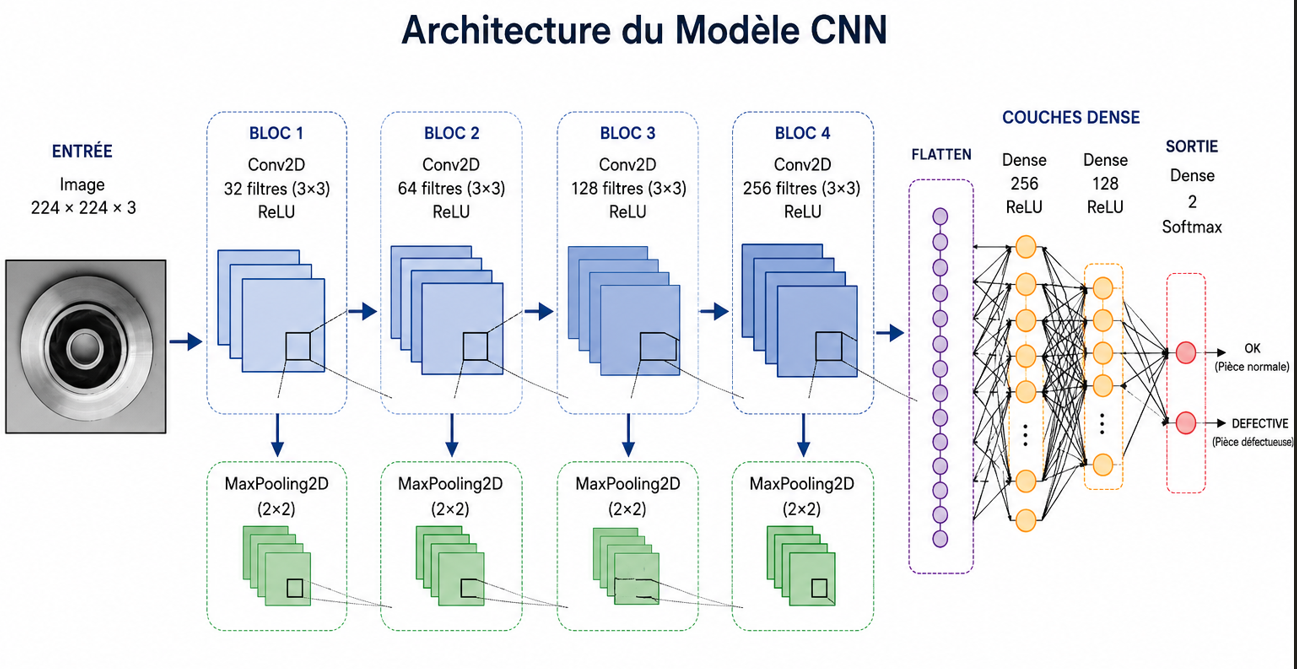
\includegraphics[width=0.8\linewidth]{archi.png}
    \caption{Architecture du CNN}
\end{figure}

\subsection{Convolution 2D}

L'opération de convolution est définie par :

\begin{equation}
(I * K)[i,j] = \sum_{m}\sum_{n} I[i+m,\, j+n] \cdot K[m,n]
\end{equation}

Tous les filtres utilisent un \textit{padding} de type \texttt{same},
préservant les dimensions spatiales à travers chaque couche convolutive
avant le sous-échantillonnage.

\subsubsection{Activation ReLU}

La fonction d'activation \term{ReLU} (\textit{Rectified Linear Unit}) est
utilisée pour introduire la non-linéarité :

\begin{equation}
\text{ReLU}(x) = \max(0, x)
\end{equation}

Son avantage principal est de ne pas saturer pour les grandes valeurs positives,
limitant le problème du gradient qui s'éteint (\textit{vanishing gradient}).

\subsubsection{MaxPooling}

Chaque bloc se termine par un sous-échantillonnage spatial $2 \times 2$ par
maximum local, réduisant de moitié les dimensions spatiales tout en conservant
les caractéristiques les plus saillantes :

\begin{equation}
\text{Sortie}_{i,j} = \max_{(p,q) \in \mathcal{P}_{i,j}} x_{p,q}
\end{equation}

Après les quatre blocs, les cartes de caractéristiques ont des dimensions
$14 \times 14 \times 256$.

\section{Classifieur dense}

La tête de classification comprend deux couches denses avec régularisation,
suivies d'une sortie \term{softmax} :

\begin{align}
h_1 &= \text{ReLU}(\text{}(W_1 \cdot \text{Flatten}(x) + b_1)) \\
h_2 &= \text{ReLU}(\text{}(W_2 \cdot h_1 + b_2)) \\
\hat{y} &= \text{softmax}(W_3 \cdot h_2 + b_3)
\end{align}

La sortie \texttt{softmax} fournit une distribution de probabilité sur les
deux classes :

\begin{equation}
\text{softmax}(z_i) = \frac{e^{z_i}}{\sum_{j} e^{z_j}}
\end{equation}


\section{Régularisation du Modèle}
% =============================================================

\subsection{Stratégies de régularisation employées}

Le premier modèle (\model{CNN\_REG}) intègre deux techniques de régularisation
complémentaires : la \term{Batch Normalization} et le \term{Dropout}.

\subsection{Batch Normalization}

la Batch Normalization
normalise les activations de chaque couche par lot pendant l'entraînement :

\begin{equation}
\hat{x}^{(k)} = \frac{x^{(k)} - \mu_{\mathcal{B}}^{(k)}}{\sqrt{\sigma_{\mathcal{B}}^{(k)2} + \epsilon}}
\end{equation}

puis applique une transformation affine apprise :

\begin{equation}
y^{(k)} = \gamma^{(k)} \hat{x}^{(k)} + \beta^{(k)}
\end{equation}

\textbf{Avantages dans ce contexte :}
\begin{itemize}
  \item Accélère la convergence en réduisant le \term{covariate shift} interne ;
  \item Agit comme régularisateur implicite, réduisant le besoin de Dropout
        dans les couches convolutives ;
  \item Permet l'utilisation de taux d'apprentissage plus élevés.
\end{itemize}

La Batch Normalization est appliquée \textbf{après} chaque couche convolutive et \textbf{après}
les couches denses, avant l'activation (pattern BN-avant-activation).

\subsection{Dropout}

Le Dropout désactive aléatoirement des neurones pendant
l'entraînement avec une probabilité $p$, forçant le réseau à apprendre des
représentations redondantes et robustes 
\begin{table}[H]
\centering
\caption{Paramètres de Dropout dans le classifieur}
\label{tab:dropout}
\begin{tabular}{|l|c|p{8cm}|}
\toprule
\textbf{Couche} & \textbf{Taux de Dropout} & \textbf{Justification} \\
\midrule
Dense(256) & $p = 0{,}5$ & Fort : couche la plus dense, risque élevé de sur-apprentissage \\
\hline
Dense(128) & $p = 0{,}3$ & Modéré : couche intermédiaire \\
\bottomrule
\end{tabular}
\end{table}


\subsection{Code complet (Modèle CNN régularisé)}

\begin{figure}[H]
\centering
    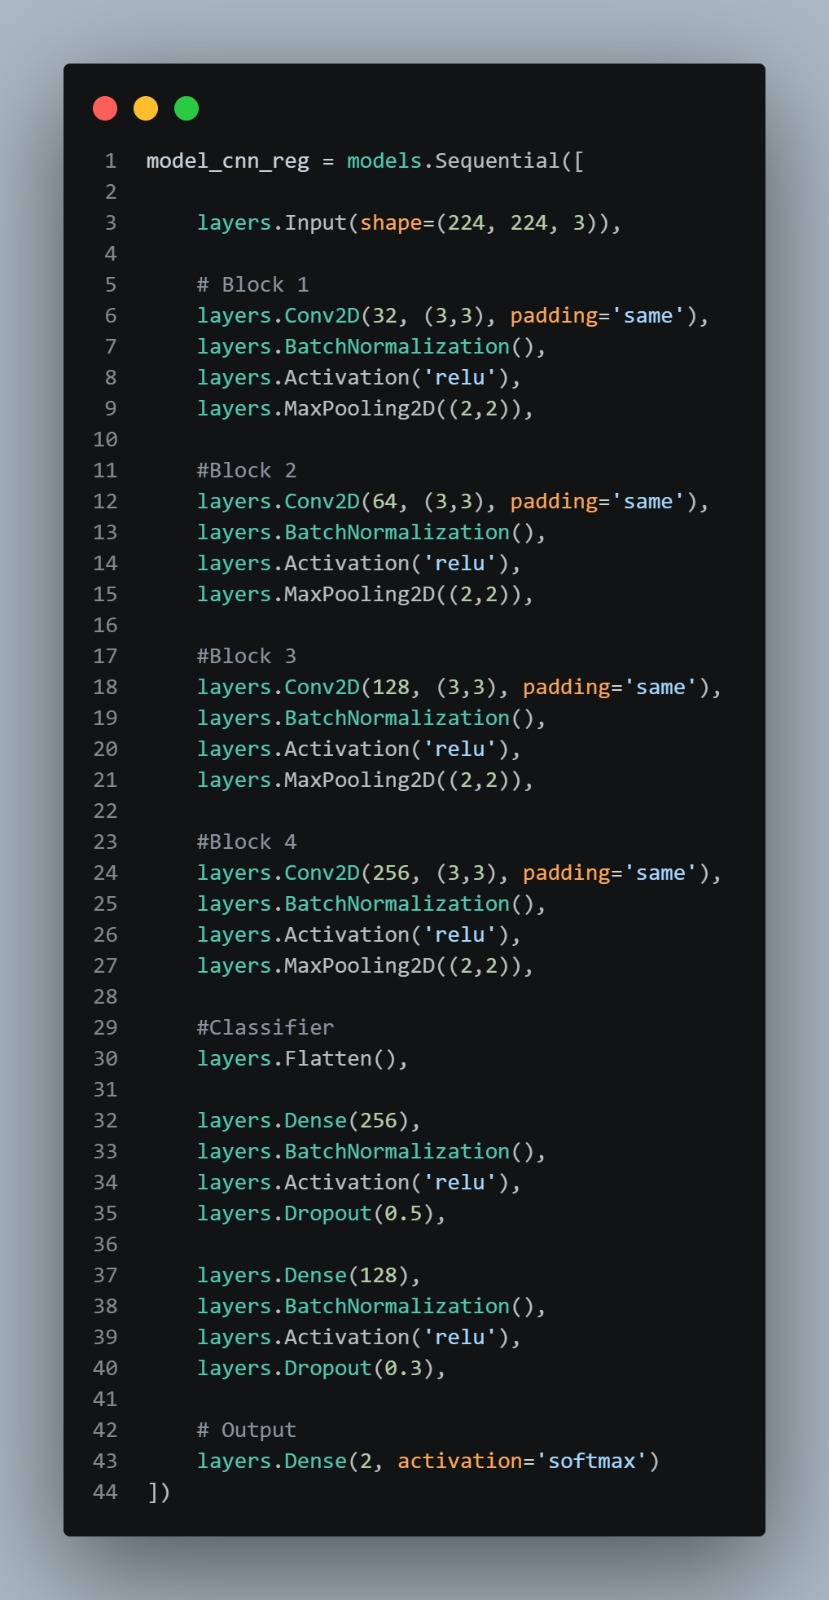
\includegraphics[width=0.8\linewidth]{code1.jpeg}
    \caption{}
\end{figure}


\newpage

\section{Récapitulatif de l'architecture}






\begin{table}[H]
\centering
\caption{Récapitulatif complet de l'architecture CNN régularisé}
\label{tab:archi}
\renewcommand{\arraystretch}{1.3}
\begin{tabular}{|c|l|c|c|}
\hline
\textbf{Bloc} & \textbf{Couche} & \textbf{Filtres / Unités} & \textbf{Sortie} \\
\hline
Input & Input & --- & $224 \times 224 \times 3$ \\
\hline
\multirow{1}
    & Conv2D    & $32,\ 3\times3$ & $224\times224\times32$ \\
    & BatchNorm & ---             & $224\times224\times32$ \\
    & ReLU      & ---             & $224\times224\times32$ \\
    & MaxPool2D & $2\times2$      & $112\times112\times32$ \\
\hline
\multirow{2}
    & Conv2D    & $64,\ 3\times3$ & $112\times112\times64$ \\
    & BatchNorm & ---             & $112\times112\times64$ \\
    & ReLU      & ---             & $112\times112\times64$ \\
    & MaxPool2D & $2\times2$      & $56\times56\times64$   \\
\hline
\multirow{3}
    & Conv2D    & $128,\ 3\times3$ & $56\times56\times128$ \\
    & BatchNorm & ---              & $56\times56\times128$ \\
    & ReLU      & ---              & $56\times56\times128$ \\
    & MaxPool2D & $2\times2$       & $28\times28\times128$ \\
\hline
\multirow{4}
    & Conv2D    & $256,\ 3\times3$ & $28\times28\times256$ \\
    & BatchNorm & ---              & $28\times28\times256$ \\
    & ReLU      & ---              & $28\times28\times256$ \\
    & MaxPool2D & $2\times2$       & $14\times14\times256$ \\
\hline
--- & Flatten   & ---    & $50\,176$ \\
\hline
\multirow{FC}
    & Dense          & 256       & 256 \\
    & BatchNorm+ReLU & ---       & 256 \\
    & Dropout        & $p=0{,}5$ & 256 \\
    & Dense          & 128       & 128 \\
    & BatchNorm+ReLU & ---       & 128 \\
    & Dropout        & $p=0{,}3$ & 128 \\
\hline
Output & Dense (softmax) & 2 & 2 \\
\hline
\end{tabular}
\end{table}






\newpage

\section{Méthodologie d'Entraînement}

\subsection{Fonction de perte}

La fonction de perte utilisée est la \term{Cross-Entropie Catégorielle
Parcimonieuse} (\textit{Sparse Categorical Cross-Entropy}), adaptée aux
labels entiers :

\begin{equation}
\mathcal{L}(\theta) = -\frac{1}{N}\sum_{i=1}^{N} \log \hat{y}_{i, y_i}
\end{equation}

où $\hat{y}_{i, y_i}$ est la probabilité prédite pour la vraie classe $y_i$
de l'exemple $i$.

\subsection{Optimiseur}

L'algorithme \textbf{Adam} est choisi pour ses propriétés
de convergence adaptative. Il combine les avantages de RMSProp (adaptation
du taux d'apprentissage par paramètre) et Momentum 



\subsection{Stratégie d'arrêt précoce}

L'\term{Early Stopping} est mis en place pour interrompre l'entraînement
dès que la performance sur le jeu de validation stagne, prévenant le
sur-apprentissage

\begin{figure}[H]
\centering
    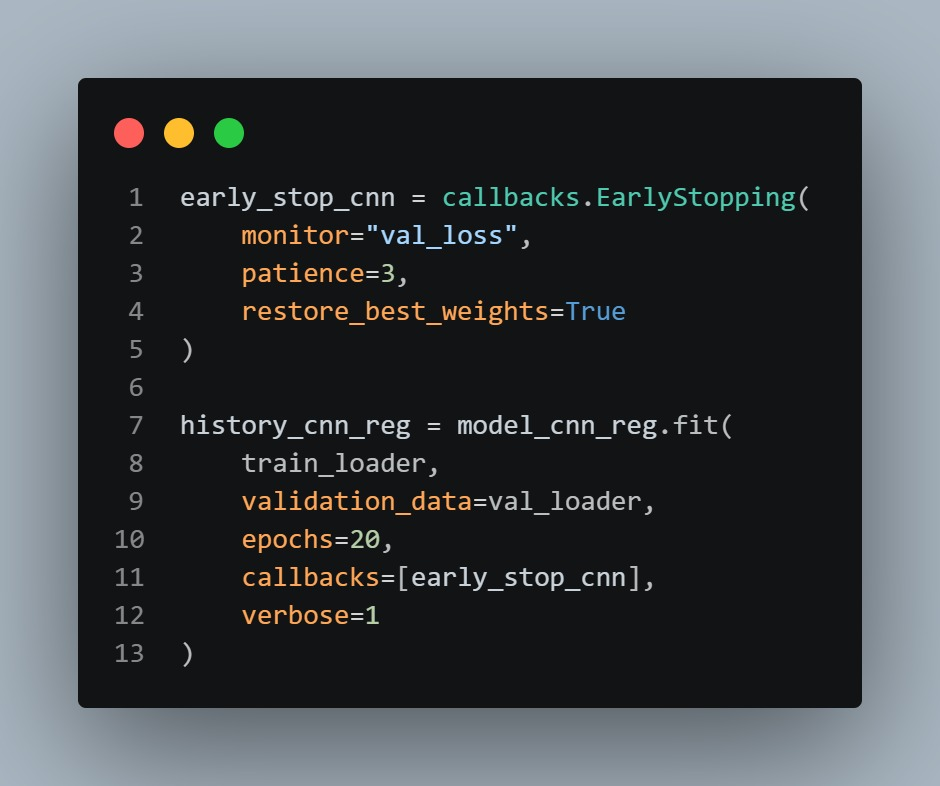
\includegraphics[width=0.8\linewidth]{code2.jpeg}
    \caption{Architecture du CNN}
\end{figure}


\subsection{Paramètres d’entraînement récapitulatifs}

\begin{table}[H]
\centering
\caption{Hyperparamètres d'entraînement communs aux deux modèles}
\label{tab:hyperparam}
\begin{tabular}{|l|l|}
\hline
\textbf{Hyperparamètre} & \textbf{Valeur} \\
\hline
Optimiseur        & Adam  \\
\hline
Fonction de perte & Sparse Categorical Cross-Entropy \\
\hline
Métrique          & Accuracy \\
\hline
Batch size        & 32 \\
\hline
Époques max       & 20 \\
\hline
Résolution        & $224 \times 224 \times 3$ \\
\hline


\end{tabular}
\end{table}


\section{Modèle CNN sans Augmentation — Résultats}

\subsection{Courbes d'apprentissage}

Les courbes d'apprentissage illustrent
l'évolution de la précision et de la perte sur les ensembles
d'entraînement et de validation au fil des époques.

\begin{figure}[H]
\centering
    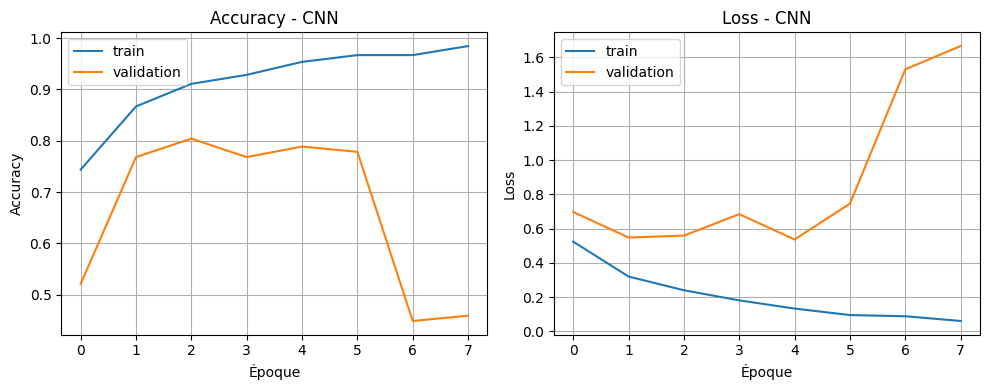
\includegraphics[width=0.8\linewidth]{code3.png}
    \caption{Courbes d'apprentissage}
\end{figure}

\subsection{Lecture des courbes}
- La courbe train (bleue) progresse de manière régulière et quasi-monotone, partant de ~0,74 à l'époque 0 pour atteindre ~0,97 à l'époque 7.

- La courbe validation (orange) démarre à ~0,52, monte rapidement jusqu'à ~0,80 aux époques 2–3, se stabilise autour de 0,78–0,80 jusqu'à l'époque 5, puis s'effondre brutalement à ~0,45 aux époques 6–7.

- La loss d'entraînement (bleue) décroît de façon continue et régulière, de ~0,55 à quasi 0,05 à l'époque 7, une descente quasi-parfaite.

- La loss de validation (orange) oscille entre 0,55 et 0,65 jusqu'à l'époque 4, puis diverge fortement pour atteindre ~1,65 à l'époque 7.

\subsection{Interprétation :}

- Le creusement progressif entre les deux courbes à partir de l'époque 3 est un signal clair de sur-apprentissage (overfitting) : le modèle mémorise les données d'entraînement sans généraliser.

- L'effondrement brutal de la validation aux époques 6–7 confirme que le modèle a dépassé son optimum de généralisation bien avant la fin de l'entraînement.

- La divergence entre la loss train et la loss validation à partir de l'époque 5 est le symptôme classique du sur-apprentissage : la perte d'entraînement continue de baisser alors que la perte de validation explose.

- Le minimum de la loss de validation se situe vers l'époque 4 (~0,57), confirmant que c'est le point optimal d'arrêt.

- La forte amplitude des oscillations sur la courbe de validation (notamment la chute aux époques 6–7 sur l'accuracy) suggère une instabilité du modèle face aux données non vues, probablement amplifiée par l'absence d'augmentation de données.

\subsection{ Conclusion générale :}

Malgré la présence de Batch Normalization et de Dropout, le modèle CNN régularisé entre en sur-apprentissage dès l'époque 5, atteignant une précision de validation maximale d'environ 80\%. Ce comportement motive directement l'introduction de l'augmentation de données dans le second modèle, afin d'enrichir artificiellement la diversité des exemples d'entraînement et de retarder — voire d'éliminer — ce phénomène de sur-apprentissage.

\subsection{Résultats sur l’ensemble de test}

\begin{table}[H]
\centering
\caption{Résultats d'évaluation du modèle CNN régularisé sur l'ensemble de test}
\label{tab:test_results_reg}
\begin{tabular}{|l|c|}
\hline
\textbf{Métrique} & \textbf{Valeur} \\
\hline
Test Loss     & $62{,}29\%\\
\hline
Test Accuracy & $80{,}20\%$ \\
\hline
\end{tabular}
\end{table}

\subsection{Matrice de confusion}

\begin{figure}[H]
\centering
    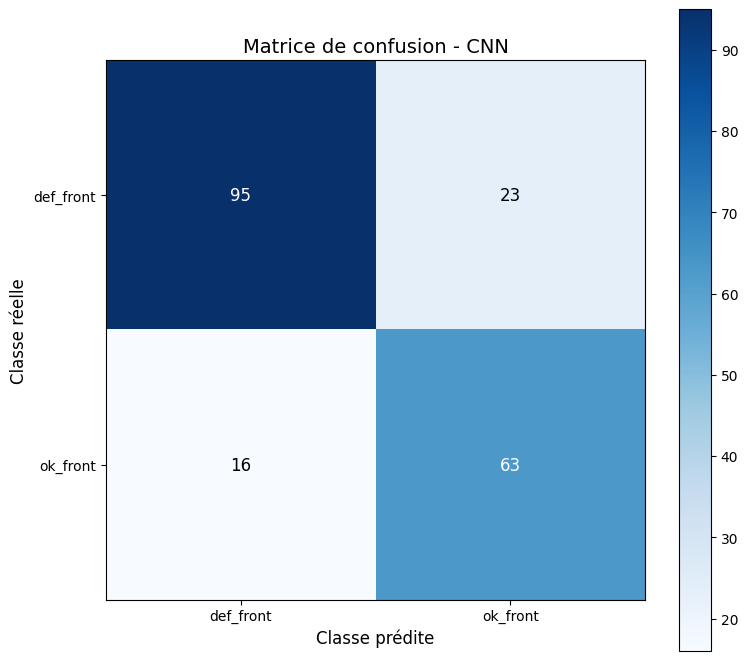
\includegraphics[width=0.8\linewidth]{code4.png}
    \caption{Matrice de confusion}
\end{figure}


La matrice de confusion permet d'analyser la
nature des erreurs du modèle. On distingue :
\begin{itemize}
  \item \textbf{Vrais Positifs (TP)} : 95 pièces défectueuses correctement identifiées.
  \item \textbf{Vrais Négatifs (TN)} : 63 pièces saines correctement identifiées.
  \item \textbf{Faux Positifs (FP)} : 16 pièces saines classées comme défectueuses.
  \item \textbf{Faux Négatifs (FN)} : 23 pièces défectueuses classées comme saines (\textit{défaut non détecté}).
\end{itemize}


\subsection{Rapport de classification}

\begin{table}[H]
\centering
\caption{Rapport de classification — CNN régularisé (sans augmentation)}
\label{tab:report_reg}
\renewcommand{\arraystretch}{1.3}
\begin{tabular}{|l|c|c|c|c|}
\hline
\textbf{Classe} & \textbf{Précision} & \textbf{Rappel} & \textbf{F1-Score} & \textbf{Support} \\
\hline
\texttt{def\_front}      & $0{,}86$ & $0{,}81$ & $0{,}83$ & 118 \\
\hline
\texttt{ok\_front}       & $0{,}73$ & $0{,}80$ & $0{,}76$ & 79  \\
\hline\hline
\textbf{Accuracy}        & \multicolumn{3}{c|}{$0{,}80$} & 197 \\
\hline
\textbf{Macro avg}       & $0{,}79$ & $0{,}80$ & $0{,}80$ & 197 \\
\hline
\textbf{Weighted avg}    & $0{,}81$ & $0{,}80$ & $0{,}80$ & 197 \\
\hline
\end{tabular}
\end{table}






\textcolor{red}{\subsubsection*{Analyse par classe}}

\textcolor{blue}{\subsubsection*{Classe \texttt{def\_front} (pièces défectueuses)}}

\begin{itemize}
    \item \textbf{Précision = 0,86} : parmi toutes les pièces prédites comme 
    défectueuses, \textbf{86\%} le sont réellement. Le modèle génère peu de 
    fausses alarmes.
    
    \item \textbf{Rappel = 0,81} : parmi les 118 pièces réellement défectueuses, 
    \textbf{81\%} sont correctement détectées. Cela signifie que \textbf{19\% 
    des défauts passent inaperçus} — soit environ 22 pièces défectueuses 
    non détectées.
    
    \item \textbf{F1-Score = 0,83} : bon équilibre précision/rappel pour cette 
    classe, confirmant que le modèle gère bien la détection des défauts.
\end{itemize}

\textcolor{blue}{\subsubsection*{Classe \texttt{ok\_front} (pièces saines)}}

\begin{itemize}
    \item \textbf{Précision = 0,73} : parmi toutes les pièces prédites comme 
    saines, seulement \textbf{73\%} le sont réellement. Le taux de faux 
    négatifs est donc notable.
    
    \item \textbf{Rappel = 0,80} : parmi les 79 pièces réellement saines, 
    \textbf{80\%} sont correctement identifiées.
    
    \item \textbf{F1-Score = 0,76} : performance modérée, inférieure à celle 
    de la classe défectueuse, révélant une \textbf{asymétrie dans les capacités 
    discriminantes} du modèle.
\end{itemize}

\textcolor{red}{\subsubsection*{Analyse du déséquilibre entre classes}}

\begin{table}[H]
\centering
\renewcommand{\arraystretch}{1.3}
\begin{tabular}{|l|c|c|}
\hline
                   & \texttt{def\_front} & \texttt{ok\_front} \\
\hline
\textbf{Support}   & 118                 & 79                 \\
\hline
\textbf{F1-Score}  & $0{,}83$            & $0{,}76$           \\
\hline
\end{tabular}
\end{table}

Le dataset est \textbf{déséquilibré} : 118 échantillons défectueux contre 
79 sains (ratio $\approx 60/40$). Ce déséquilibre explique en partie pourquoi 
le modèle performe mieux sur la classe majoritaire \texttt{def\_front}. 
La classe minoritaire \texttt{ok\_front} souffre d'une précision plus faible 
($0{,}73$), le modèle ayant tendance à sur-prédire la classe défectueuse.

\textcolor{red}{\subsubsection*{Analyse des métriques globales}}

\begin{itemize}
    \item \textbf{Accuracy = 0,80} : le modèle classe correctement \textbf{80\%} 
    des 197 échantillons de test. C'est une performance acceptable mais 
    perfectible pour un système de contrôle qualité industriel.

    \item \textbf{Macro avg (0,79 / 0,80 / 0,80)} : moyenne non pondérée des 
    deux classes. Le score équilibré entre précision et rappel indique que le 
    modèle ne néglige pas complètement la classe minoritaire, mais l'écart de 
    F1 ($0{,}83$ vs $0{,}76$) reste préoccupant.

    \item \textbf{Weighted avg (0,81 / 0,80 / 0,80)} : moyenne pondérée par 
    le support. Légèrement supérieure à la macro avg en précision ($0{,}81$ 
    vs $0{,}79$), ce qui confirme l'influence de la classe majoritaire 
    \texttt{def\_front} sur les performances globales.
\end{itemize}

\subsection*{Conclusion et perspective industrielle}

\begin{tcolorbox}[colback=orange!5, colframe=orange!80!black]
Le modèle CNN régularisé présente un \textbf{profil de performance asymétrique} : 
il détecte bien les défauts (F1 $= 0{,}83$) mais est moins fiable pour valider 
les pièces saines (F1 $= 0{,}76$). Dans un contexte industriel, les 
\textbf{19\% de défauts non détectés} (rappel \texttt{def\_front} $= 0{,}81$) 
représentent le point critique à améliorer en priorité, car laisser passer 
une pièce défectueuse est bien plus coûteux qu'une fausse alarme. Ces résultats 
motivent directement l'introduction de \textbf{l'augmentation de données} dans 
le second modèle, afin d'améliorer le rappel sur la classe défectueuse et de 
réduire l'asymétrie entre les deux classes.
\end{tcolorbox}

\newpage
\section{Modèle CNN avec Augmentation de Données}

Le modèle \model{CNN\_AUG} partage la même topologie de base mais sans
Batch Normalization dans les blocs convolutifs, l'augmentation de données
jouant le rôle de régularisateur principal.




\begin{figure}[H]
\centering
    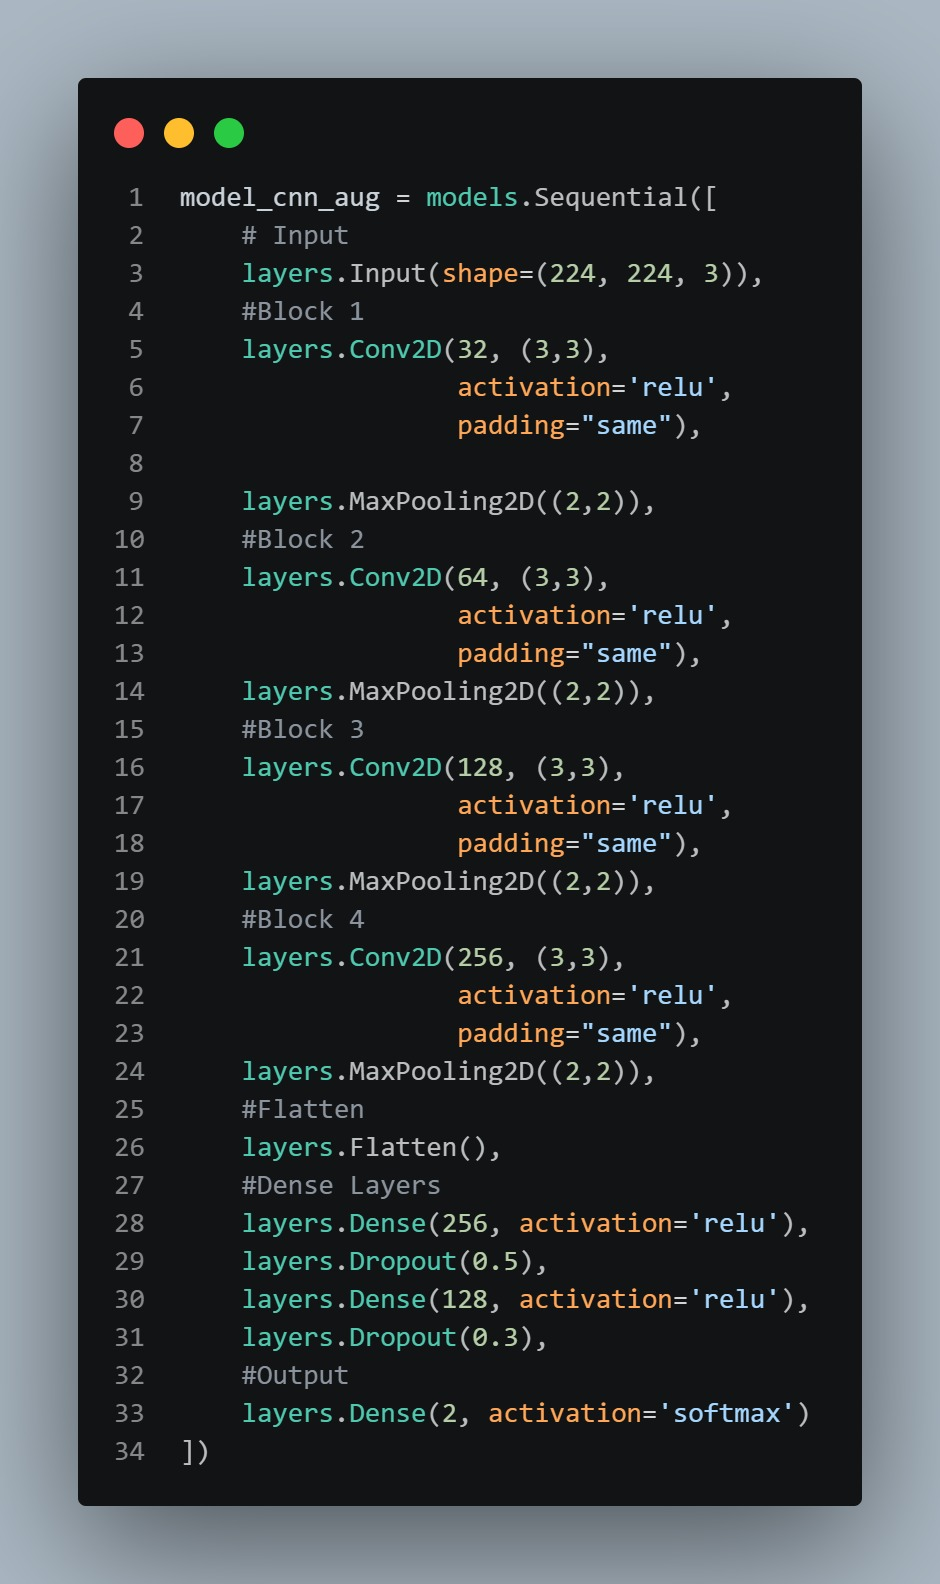
\includegraphics[width=0.8\linewidth]{code5.jpeg}
    \caption{Matrice de confusion}
\end{figure}


\begin{table}[H]
\centering
\caption{Comparaison des architectures CNN\_REG vs CNN\_AUG}
\label{tab:arch_comparison}
\renewcommand{\arraystretch}{1.3}
\begin{tabular}{|l|c|c|}
\hline
\textbf{Composant} & \textbf{CNN\_REG} & \textbf{CNN\_AUG} \\
\hline
Blocs Conv (×4)          & Conv + BN + ReLU + MaxPool & Conv + ReLU + MaxPool \\
\hline
Couches denses           & Dense + BN + ReLU          & Dense + ReLU          \\
\hline
Dropout                  & $0{,}5$ et $0{,}3$         & $0{,}5$ et $0{,}3$    \\
\hline
Batch Normalization      & oui                     & non                \\
\hline
Augmentation de données  & non                     & oui (12 transformations) \\
\hline
Early stopping patience  & 3                          & 5                     \\
\hline
\end{tabular}
\end{table}


\subsection{Courbes d'apprentissage}

\begin{figure}[H]
\centering
    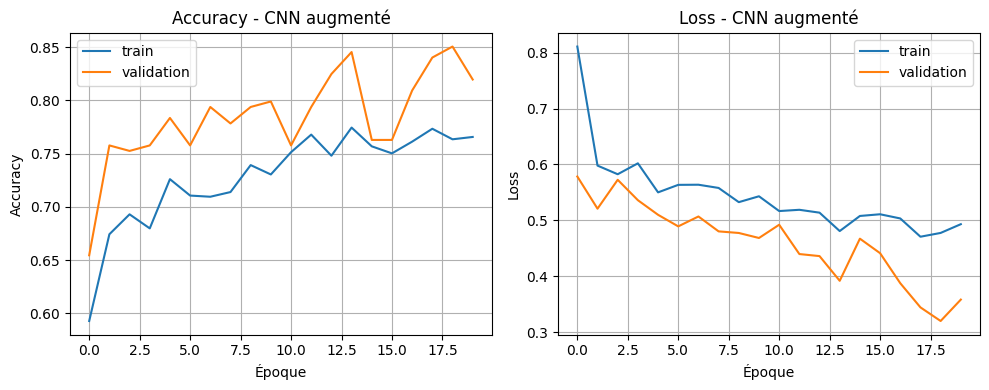
\includegraphics[width=0.8\linewidth]{code6.png}
    \caption{Courbes d'apprentissage}
\end{figure}

\subsubsection{Lecture des courbes}
- La courbe train (bleue) démarre à ~0,60 à l'époque 0, progresse lentement et de manière irrégulière, pour atteindre ~0,77 à l'époque 19.

- La courbe validation (orange) démarre plus haut à ~0,65, oscille entre 0,75 et 0,85 tout au long de l'entraînement, avec un pic maximal de ~0,85 vers l'époque 13–14, avant de légèrement redescendre à ~0,82 en fin d'entraînement.

- La loss d'entraînement (bleue) démarre à ~0,80, décroît progressivement avec des oscillations, pour se stabiliser autour de ~0,49 à l'époque 19.

- La loss de validation (orange) démarre à ~0,58, décroît de manière plus régulière et plus rapide que la loss d'entraînement, atteignant un minimum de ~0,32 vers l'époque 18–19.

\subsubsection{Interprétation :}

- Le phénomène le plus remarquable est que la courbe de validation est systématiquement supérieure à la courbe d'entraînement sur la quasi-totalité des époques. Ceci est un comportement inverse du sur-apprentissage classique, directement causé par l'augmentation de données : les images d'entraînement sont présentées sous des formes aléatoirement transformées (flips, rotations, jitter colorimétrique, etc.), rendant la tâche d'entraînement artificiellement plus difficile que l'évaluation sur des images non augmentées.

- La progression lente et irrégulière de la courbe train (oscillations) est également caractéristique de l'augmentation stochastique : chaque époque présente des exemples différents, introduisant de la variance dans le gradient.

- L'absence de divergence entre les deux courbes confirme que le sur-apprentissage est bien contrôlé grâce à l'augmentation.

- Comme pour l'accuracy, la loss de validation est inférieure à la loss d'entraînement sur toute la durée, confirmant l'effet de l'augmentation qui rend l'entraînement plus difficile que l'évaluation.

- La décroissance continue et régulière de la loss de validation, sans divergence ni remontée brutale (contrairement au modèle sans augmentation), est le signe d'une généralisation saine et stable.

- L'écart croissant entre les deux courbes de loss en fin d'entraînement indique que le modèle continue d'apprendre et de progresser sans saturer, suggérant qu'un entraînement plus long (au-delà de 20 époques) pourrait encore améliorer les performances.

\subsubsection{ Conclusion générale :}

Les courbes d'apprentissage du CNN augmenté présentent un profil radicalement différent du modèle sans augmentation. L'augmentation de données remplit parfaitement son rôle de régularisateur fonctionnel : elle élimine le sur-apprentissage, stabilise la validation sur 20 époques et permet d'atteindre une accuracy de 84,26\% contre 80,20\% pour le modèle précédent. En contrepartie, la convergence est plus lente et nécessite davantage d'époques, justifiant la patience d'Early Stopping portée à 5 pour ce modèle.


\subsection{Résultats sur l'ensemble de test}

\begin{table}[H]
\centering
\caption{Résultats d'évaluation du modèle CNN avec augmentation sur l'ensemble de test}
\label{tab:test_results_aug}
\begin{tabular}{|l|c|}
\hline
\textbf{Métrique} & \textbf{Valeur} \\
\hline
Test Loss     & $31{,}68\%$ \\
\hline
Test Accuracy & $84{,}26\%$ \\
\hline
\end{tabular}
\end{table}

\subsection{Matrice de confusion}
\begin{figure}[H]
\centering
    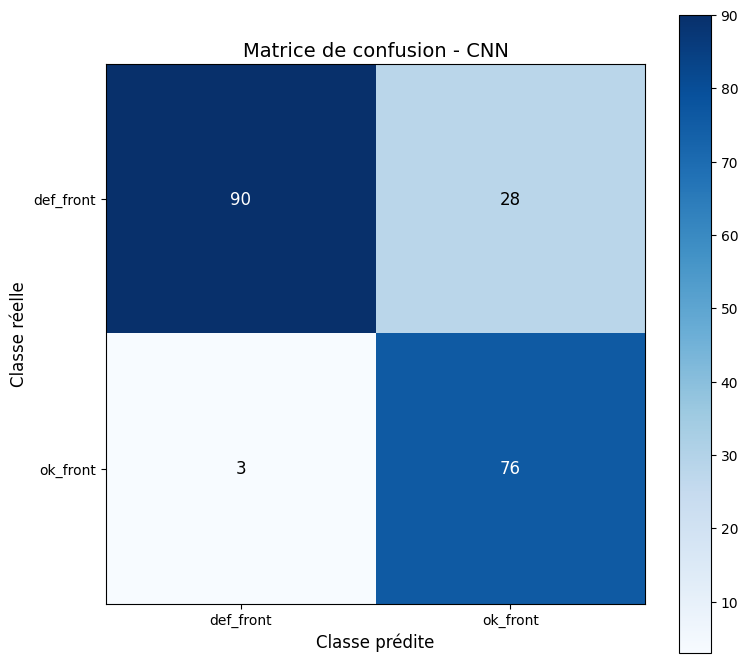
\includegraphics[width=0.8\linewidth]{code7.png}
    \caption{Matrice de confusion du modèle CNN avec augmentation des données}
\end{figure}

\subsection{Rapport de classification}

\begin{table}[H]
\centering
\caption{Rapport de classification — CNN avec augmentation de données}
\label{tab:report_aug}
\renewcommand{\arraystretch}{1.3}
\begin{tabular}{|l|c|c|c|c|}
\hline
\textbf{Classe} & \textbf{Précision} & \textbf{Rappel} & \textbf{F1-Score} & \textbf{Support} \\
\hline
\texttt{def\_front}      & $0{,}97$ & $0{,}76$ & $0{,}85$ & 118 \\
\hline
\texttt{ok\_front}       & $0{,}73$ & $0{,}96$ & $0{,}83$ & 79  \\
\hline\hline
\textbf{Accuracy}        & \multicolumn{3}{c|}{$0{,}84$} & 197 \\
\hline
\textbf{Macro avg}       & $0{,}85$ & $0{,}86$ & $0{,}84$ & 197 \\
\hline
\textbf{Weighted avg}    & $0{,}87$ & $0{,}84$ & $0{,}84$ & 197 \\
\hline
\end{tabular}
\end{table}

% =============================================================
\section{Comparaison des Deux Modèles}
% =============================================================

\begin{table}[H]
\centering
\caption{Comparaison des performances finales sur l'ensemble de test}
\label{tab:comparison}
\renewcommand{\arraystretch}{1.4}
\begin{tabular}{|l|c|c|}
\hline
\textbf{Critère} & \textbf{CNN régularisé} & \textbf{CNN + Augmentation} \\
\hline
Accuracy test               & $80{,}20\%$         & $84{,}26\%$ \\
\hline
Amélioration absolue        & ---                 & $+4{,}06$ pp \\
\hline
Amélioration relative       & ---                 & $+5{,}06\%$ \\
\hline
Régularisation structurelle & BN + Dropout        & Dropout seulement \\
\hline
Augmentation de données     & Non                 & Oui (12 transformations) \\
\hline
Early stopping patience     & 3                   & 5 \\
\hline
\end{tabular}
\end{table}


\subsection{Visualisation comparative}


\begin{figure}[H]
\centering
    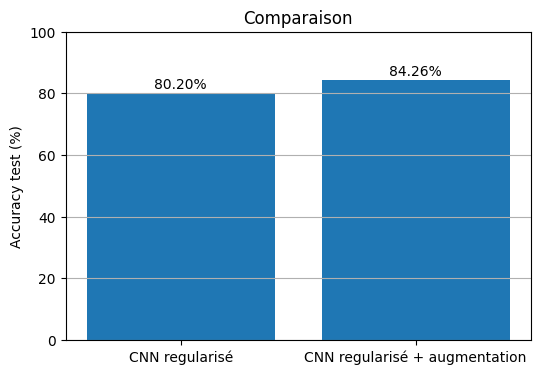
\includegraphics[width=0.8\linewidth]{code8.png}
    \caption{Comparaison des deux modèles}
\end{figure}

Le diagramme en barres  illustre clairement
l'apport de l'augmentation de données : une amélioration de
\textbf{4{,}06 pourcentage} en l'accuracy sur l'ensemble de test.


\subsection{Analyse qualitative}

\begin{table}[H]
\centering
\caption{Analyse qualitative comparative des deux approches}
\label{tab:qualitative}
\renewcommand{\arraystretch}{1.3}
\begin{tabular}{|p{5cm}|p{4.5cm}|p{4.5cm}|}
\hline
\textbf{Aspect} & \textbf{CNN régularisé} & \textbf{CNN + Augmentation} \\
\hline
Régularisation & BN comme régularisateur implicite fort & Augmentation comme régularisateur externe \\
\hline
Vitesse de convergence & Rapide (BN) & Plus lente (variabilité aug.) \\
\hline
Stabilité validation & Bonne & Très bonne \\
\hline
Robustesse aux perturbations & Modérée & Haute \\
\hline
Coût computationnel & Modéré & Plus élevé (aug. en ligne) \\
\hline
Performance finale & $80{,}20\%$ & $84{,}26\%$ \\
\hline
\end{tabular}
\end{table}
\section{Discussion}

L'amélioration de \textbf{+4{,}06\%} apportée par l'augmentation de données
peut s'expliquer par plusieurs mécanismes :

\begin{enumerate}
  \item \textbf{Augmentation artificielle de la diversité} : chaque image est
        présentée sous des centaines de variantes au fil des époques, forçant
        le réseau à apprendre des caractéristiques invariantes à l'orientation,
        l'éclairage et la couleur ;

  \item \textbf{Spécificité industrielle des transformations} : les transformations
        comme l'AWB, l'égalisation d'histogramme et le channel shuffle ont été
        conçues pour refléter les conditions réelles d'acquisition d'images en
        usine (variabilité de l'éclairage, caméras différentes) ;

  \item \textbf{Réduction du sur-apprentissage} : l'augmentation agit comme un
        régularisateur fonctionnel qui complète le Dropout, rendant le modèle
        moins sensible aux artefacts spécifiques du jeu d'entraînement.
\end{enumerate}

% =====================================================================
%  EXTRAIT : Transfer Learning → Conclusion générale
%  Système Intelligent de Contrôle Qualité des Impellers
%  Filière BDIA1 - Année universitaire 2025-2026
% =====================================================================
\documentclass[12pt,a4paper,openany]{report}

% ---------- Encoding & langue ----------
\usepackage[utf8]{inputenc}
\usepackage[T1]{fontenc}
\usepackage[french]{babel}
\usepackage{lmodern}
\usepackage{microtype}

% ---------- Mise en page ----------
\usepackage[a4paper,margin=2.5cm,headheight=15pt]{geometry}
\usepackage{setspace}
\onehalfspacing
\usepackage{parskip}
\usepackage{fancyhdr}
\usepackage{titlesec}
\usepackage{enumitem}
\setlist{itemsep=2pt,topsep=4pt}

% ---------- Graphiques & tableaux ----------
\usepackage{graphicx}
\usepackage{float}
\usepackage{caption}
\usepackage{subcaption}
\captionsetup{font=small,labelfont=bf}
\graphicspath{{images/}}
\usepackage{array}
\usepackage{booktabs}
\usepackage{longtable}
\usepackage{tabularx}
\usepackage{multirow}
\usepackage{makecell}

% ---------- Couleurs ----------
\usepackage[dvipsnames]{xcolor}
\definecolor{primary}{RGB}{0,90,160}
\definecolor{accent}{RGB}{200,80,30}
\definecolor{softgray}{RGB}{240,240,245}
\definecolor{codebg}{RGB}{248,248,248}
\definecolor{codekw}{RGB}{0,90,160}
\definecolor{codestr}{RGB}{170,55,30}
\definecolor{codecmt}{RGB}{100,110,100}

% ---------- Boites ----------
\usepackage[most]{tcolorbox}
\newtcolorbox{infobox}[1][]{enhanced,colback=softgray,colframe=primary,
  fonttitle=\bfseries,coltitle=white,colbacktitle=primary,
  boxrule=0.4pt,arc=2pt,left=8pt,right=8pt,top=4pt,bottom=4pt,#1}
\newtcolorbox{warnbox}[1][]{enhanced,colback=accent!8,colframe=accent,
  fonttitle=\bfseries,coltitle=white,colbacktitle=accent,
  boxrule=0.4pt,arc=2pt,left=8pt,right=8pt,top=4pt,bottom=4pt,#1}

% ---------- Code ----------
\usepackage{listings}
\lstdefinestyle{pystyle}{
  language=Python,
  backgroundcolor=\color{codebg},
  basicstyle=\ttfamily\footnotesize,
  keywordstyle=\color{codekw}\bfseries,
  stringstyle=\color{codestr},
  commentstyle=\color{codecmt}\itshape,
  numbers=left, numberstyle=\tiny\color{gray}, numbersep=6pt,
  frame=single, rulecolor=\color{gray!40},
  breaklines=true, breakatwhitespace=true,
  showstringspaces=false,
  tabsize=2, captionpos=b,
  literate=
    {é}{{\'e}}1 {è}{{\`e}}1 {ê}{{\^e}}1 {à}{{\`a}}1 {â}{{\^a}}1
    {î}{{\^\i}}1 {ô}{{\^o}}1 {ù}{{\`u}}1 {û}{{\^u}}1 {ç}{{\c c}}1
    {É}{{\'E}}1 {È}{{\`E}}1 {Ê}{{\^E}}1 {À}{{\`A}}1 {œ}{{\oe}}1
}
\lstset{style=pystyle}

% ---------- Mathématiques ----------
\usepackage{amsmath,amssymb,amsfonts}

% ---------- Acronymes ----------
\usepackage[acronym,nonumberlist,toc]{glossaries}
\makeglossaries

\newacronym{ia}{IA}{Intelligence Artificielle}
\newacronym{dl}{DL}{Deep Learning (apprentissage profond)}
\newacronym{ml}{ML}{Machine Learning (apprentissage automatique)}
\newacronym{cnn}{CNN}{Convolutional Neural Network}
\newacronym{mlp}{MLP}{Multi-Layer Perceptron}
\newacronym{tl}{TL}{Transfer Learning (apprentissage par transfert)}
\newacronym{cv}{CV}{Computer Vision}
\newacronym{qc}{QC}{Quality Control (contrôle qualité)}
\newacronym{cao}{CAO}{Conception Assistée par Ordinateur}
\newacronym{relu}{ReLU}{Rectified Linear Unit}
\newacronym{bn}{BN}{Batch Normalization}
\newacronym{sgd}{SGD}{Stochastic Gradient Descent}
\newacronym{lr}{LR}{Learning Rate (taux d'apprentissage)}
\newacronym{auc}{AUC}{Area Under the Curve}
\newacronym{roc}{ROC}{Receiver Operating Characteristic}
\newacronym{tpr}{TPR}{True Positive Rate}
\newacronym{fpr}{FPR}{False Positive Rate}
\newacronym{fn}{FN}{Faux Negatif}
\newacronym{fp}{FP}{Faux Positif}
\newacronym{ap}{AP}{Average Precision}
\newacronym{api}{API}{Application Programming Interface}
\newacronym{gpu}{GPU}{Graphics Processing Unit}
\newacronym{cpu}{CPU}{Central Processing Unit}
\newacronym{rgb}{RGB}{Red Green Blue}
\newacronym{tf}{TF}{TensorFlow}
\newacronym{tflite}{TFLite}{TensorFlow Lite}

% ---------- Hyperliens ----------
\usepackage[hidelinks,colorlinks=true,linkcolor=primary,urlcolor=primary,citecolor=accent]{hyperref}

% ---------- Style des chapitres / sections ----------
\titleformat{\chapter}[hang]{\Huge\bfseries\color{primary}}{\thechapter.}{1em}{}
\titlespacing*{\chapter}{0pt}{-20pt}{20pt}
\titleformat{\section}{\Large\bfseries\color{primary}}{\thesection}{0.6em}{}
\titleformat{\subsection}{\large\bfseries\color{accent}}{\thesubsection}{0.5em}{}

% ---------- En-tête / pied de page ----------
\pagestyle{fancy}
\fancyhf{}
\renewcommand{\headrulewidth}{0.4pt}
\renewcommand{\footrulewidth}{0pt}
\fancyhead[L]{\small\textit{Contrôle Qualité Intelligent des Impellers}}
\fancyhead[R]{\small\textit{BDIA1 - 2025/2026}}
\fancyfoot[C]{\thepage}

% =====================================================================
\begin{document}

% Numérotation continue depuis le document principal
\setcounter{chapter}{5}   % Chapitres 1-5 déjà écrits
\setcounter{section}{2}   % Sections 6.1 (MLP) et 6.2 (CNN) déjà écrites

% --------------------------------------------------------- TL
\section{Modèle 3 : Transfer Learning avec EfficientNetB0}

\subsection{Principe du Transfer Learning}

Le \emph{Transfer Learning} (\gls{tl}, apprentissage par transfert) consiste a \textbf{reutiliser un réseau de neurones déjà entraîne} sur une grande base d'images --- ici \textsc{ImageNet}, qui contient $\sim 1{,}2$ million d'images réparties sur $1\,000$ classes --- pour résoudre un nouveau problème plus spécifique. Ce paradigme exploite le fait que les premières couches d'un CNN apprennent des concepts visuels \emph{génériques} (contours, textures, formes) qui sont \emph{transférables} a presque toutes les tâches d'images naturelles.

\begin{figure}[H]
    \centering
    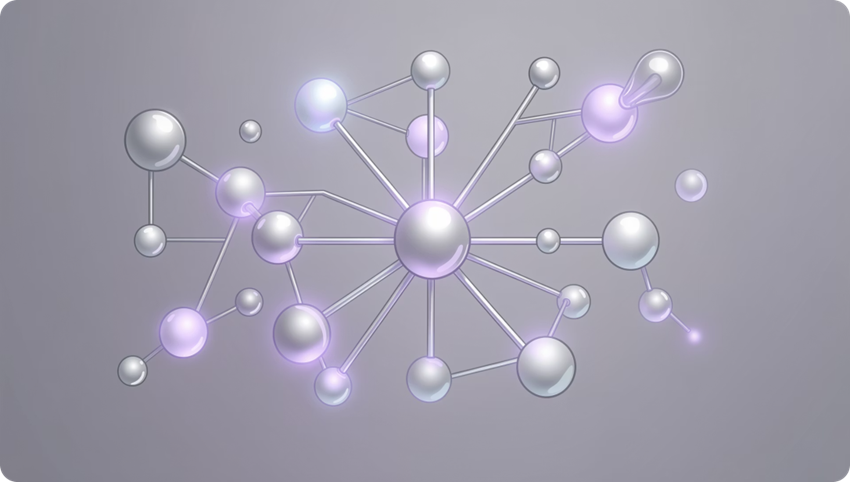
\includegraphics[width=0.85\textwidth]{image39.png}
    \caption{Principe général du Transfer Learning~: reutilisation des features d'un modèle pre-entraîne.}
    \label{fig:tlprinciple}
\end{figure}

\paragraph{Lecture de la figure~\ref{fig:tlprinciple}.}
Le schéma illustre le mécanisme de transfert~: a gauche, un réseau profond pre-entraîne sur ImageNet à déjà appris à extraire des features riches sur 1\,000 catégories de la vie courante. A droite, ce même réseau (ou ses premières couches) est reutilise comme \emph{extracteur de features} sur notre problème cible (détection de défauts), ne necessitant que l'apprentissage d'une nouvelle tête de classification spécifique. Le gain est double~: convergence plus rapide \emph{et} meilleure généralisation, car le réseau beneficie de millions d'images d'entraînement initiales.

\subsection{Stratégie en deux phases}

Notre stratégie de Transfer Learning suit le schéma canonique en \textbf{deux phases successives}~:

\begin{table}[H]
\centering
\begin{tabular}{p{4cm}p{8.5cm}}
\toprule
\textbf{Phase} & \textbf{Ce que l'on entraîne} \\
\midrule
1. Extraction de caractéristiques & \textbf{Tête de classification uniquement}~: le \emph{backbone} pre-entraîne est gele. \\[2pt]
2. \emph{Fine-tuning}              & Tête \textbf{+} dernières couches du \emph{backbone}, avec un \emph{learning rate} très faible. \\
\bottomrule
\end{tabular}
\caption{Stratégie de Transfer Learning à deux étages.}
\label{tab:tlstrategy}
\end{table}

\paragraph{Justification.}
\begin{itemize}
    \item Notre dataset est relativement petit ($\sim 6\,600$ images d'entraînement)~: entraîner un grand réseau de zero provoquerait du sur-apprentissage.
    \item Les caractéristiques visuelles génériques apprises sur ImageNet (contours, textures, formes) sont transférables à presque toute tâche d'image.
    \item La phase 1 évite de \og casser \fg\ les filtres pre-entraînés~; la phase 2 les ajuste finement à notre tâche spécifique.
\end{itemize}

\begin{figure}[H]
    \centering
    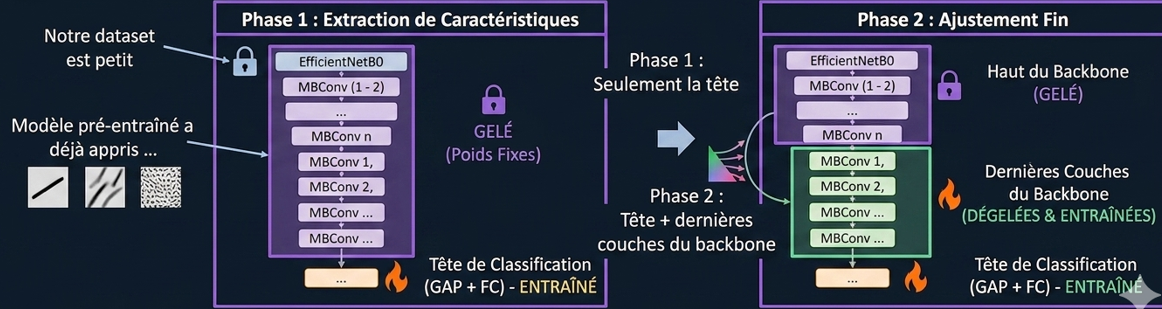
\includegraphics[width=0.85\textwidth]{image40.png}
    \caption{Reutilisation du \emph{backbone} pre-entraîne~: la tête originale (1\,000 classes ImageNet) est remplacée par une tête binaire.}
    \label{fig:tlbackbone}
\end{figure}

\paragraph{Lecture de la figure~\ref{fig:tlbackbone}.}
Le schéma montre la transformation opérée sur le réseau pre-entraîne~: on \textbf{conserve} les couches convolutives (qui constituent l'extracteur de features générique) et on \textbf{remplacé} la tête originale, prévue pour 1\,000 classes ImageNet, par une nouvelle tête adaptée à notre problème binaire. Le \emph{backbone} reste fige durant la phase 1.

\subsection{Architecture choisie : EfficientNetB0}

\textsc{EfficientNet} \cite{tan2019efficientnet} est une famille d'architectures développée par Google en 2019, dont la spécificité est de \textbf{coupler haute performance et faible coût de calcul} grace au \emph{compound scaling} déjà décrit dans l'état de l'art (chapitre 2). Le modèle \textsc{EfficientNetB0}, a la base de la famille, compte 5{,}3 millions de paramètres et atteint $77{,}3\%$ de top-1 accuracy sur ImageNet --- excellent compromis pour le Transfer Learning sur dataset modéré.

\begin{figure}[H]
    \centering
    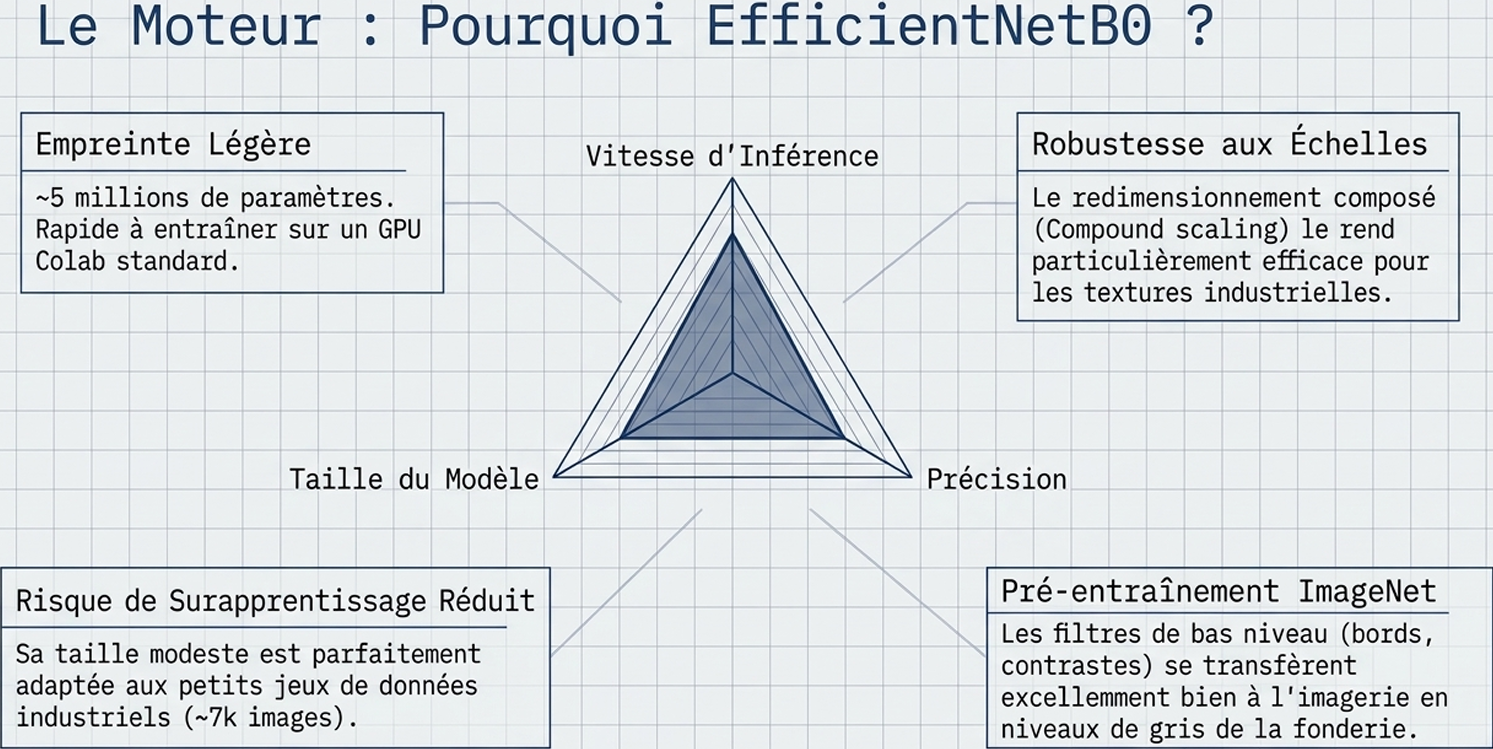
\includegraphics[width=0.92\textwidth]{image41.png}
    \caption{Architecture détaillée d'EfficientNetB0 (blocs MBConv).}
    \label{fig:efficientnet}
\end{figure}

\paragraph{Lecture de la figure~\ref{fig:efficientnet}.}
L'architecture s'articule autour de blocs \textsc{MBConv} (\emph{Mobile Inverted Bottleneck}) avec mécanismes \emph{Squeeze-and-Excitation}. La séquence de blocs alterne diverses tailles de filtres ($3\times 3$, $5\times 5$) et facteurs d'expansion. La fin du backbone produit un tenseur de features dimensionne $7\times 7\times 1280$, qui sera ensuite condensé par un \emph{Global Average Pooling} avant d'entrer dans la tête de classification.

\subsection{Source des données et preparation}

Le dataset utilisé pour cette expérience est la \textbf{version augmentée} fournie directement par l'auteur sur Kaggle, déjà adaptée aux contraintes industrielles (variations d'éclairage, angles, textures de surface). Notre prétraitement se limite donc au redimensionnement et à la normalisation requise par EfficientNetB0.

\begin{figure}[H]
    \centering
    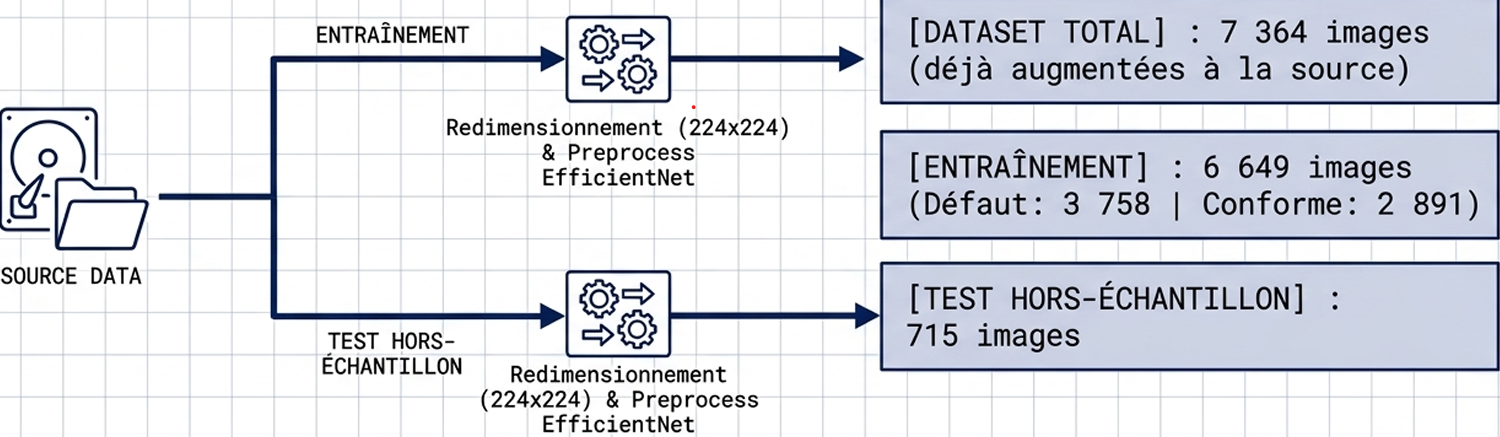
\includegraphics[width=0.92\textwidth]{image42.png}
    \caption{Dataset \emph{Casting Defect Détection} dans sa version augmentée fournie sur Kaggle.}
    \label{fig:datasetkaggle}
\end{figure}

\paragraph{Lecture de la figure~\ref{fig:datasetkaggle}.}
On observe la diversité des exemples fournis, avec variations d'angle, de zoom et de luminosite. Cette diversité est precieuse car elle permet au modèle d'apprendre des représentations robustes \emph{sans qu'il nous soit nécessaire d'ajouter une augmentation manuelle supplémentaire}. Le travail de l'auteur du dataset constitue donc une vraie valeur ajoutée.

\paragraph{Chargement automatique.}
Keras lit automatiquement l'arborescence \texttt{train/ok\_front/} et \texttt{train/def\_front/}, redimensionne en $224\times224$ et attribue un label binaire en conséquence. La fonction \texttt{preprocess\_input} d'EfficientNet transforme ensuite les valeurs $[0, 255]$ vers $[-1, 1]$ (centrage attendu par le backbone).

\begin{figure}[H]
    \centering
    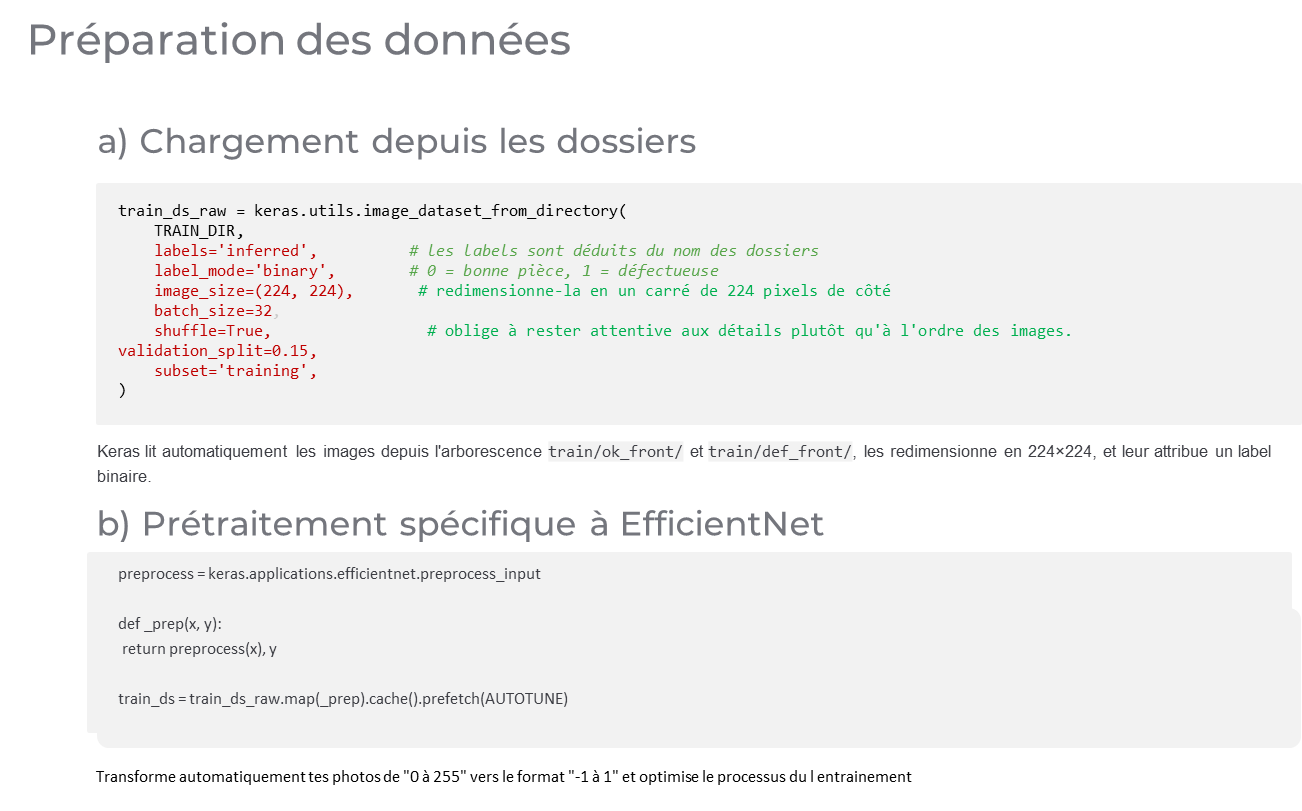
\includegraphics[width=0.95\textwidth]{image43.png}
    \caption{Code de chargement et de prétraitement adapté à EfficientNet.}
    \label{fig:loadcode}
\end{figure}

\paragraph{Lecture de la figure~\ref{fig:loadcode}.}
Le code utilisé \texttt{tf.keras.preprocessing.image\_dataset\_from\_directory} pour le chargement automatique, suivi de \texttt{efficientnet.preprocess\_input} pour la normalisation. Cette approche \emph{declarative} réduit le risque d'erreurs de prétraitement et garantit la cohérence avec les attentes du backbone pre-entraîne.

\subsection{Hyperparamètres}

\begin{figure}[H]
    \centering
    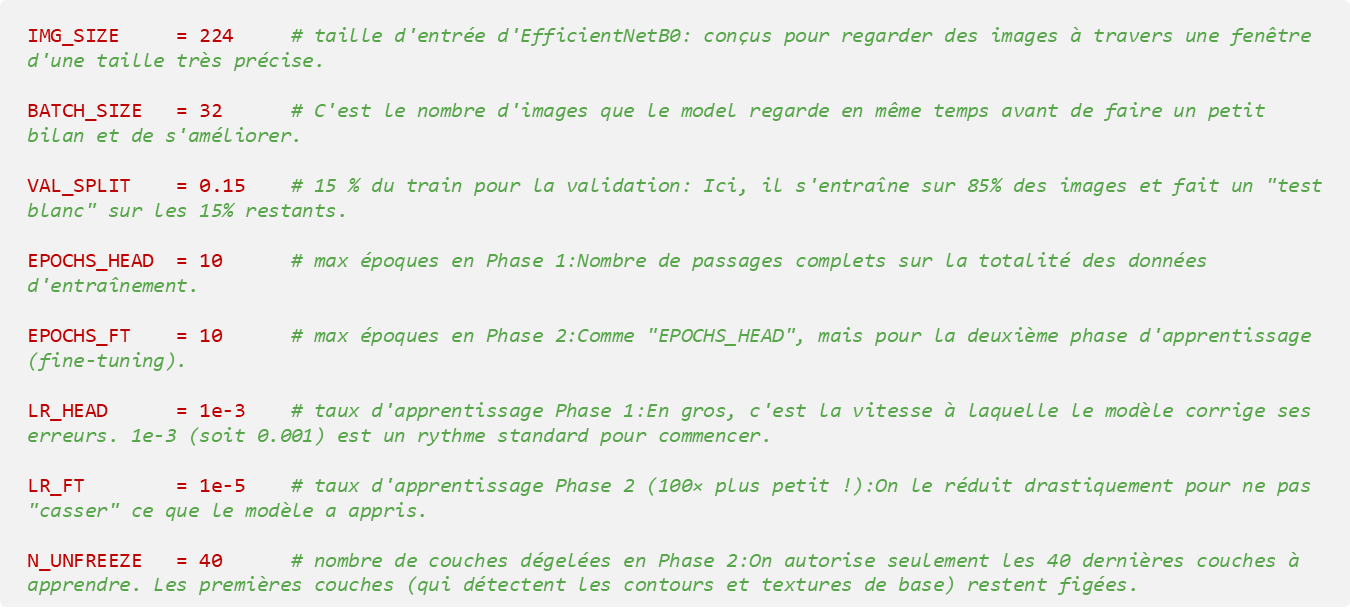
\includegraphics[width=0.95\textwidth]{image44.png}
    \caption{Hyperparamètres clés utilisés pour les deux phases.}
    \label{fig:hyperparams}
\end{figure}

\paragraph{Lecture de la figure~\ref{fig:hyperparams}.}
Les hyperparamètres distinguent clairement les deux phases~: la phase 1 utilisé un \emph{learning rate} relativement élevé ($10^{-3}$) car seule la tête de classification est entraînée --- elle peut supporter un grand pas d'apprentissage. La phase 2, en revanche, utilisé un LR très faible ($10^{-5}$) pour ajuster finement les filtres pre-entraînés sans les détruire. Ce choix d'un LR trois ordres de grandeur plus petit est la \textbf{règle d'or} du fine-tuning.

\subsection{Construction du modèle}

On conserve le \emph{backbone} EfficientNetB0 sans son classificateur d'origine, et on le \textbf{verrouille} (\texttt{trainable = False}) pour préserver le savoir acquis sur ImageNet. Les cartes de caractéristiques sont condensées par un \emph{Global Average Pooling}, suivies d'un \texttt{Dropout} pour la régularisation, et d'une couche \texttt{Dense(1)} avec activation \emph{sigmoid} pour la prédiction binaire.

\begin{figure}[H]
    \centering
    \begin{subfigure}{0.65\textwidth}
        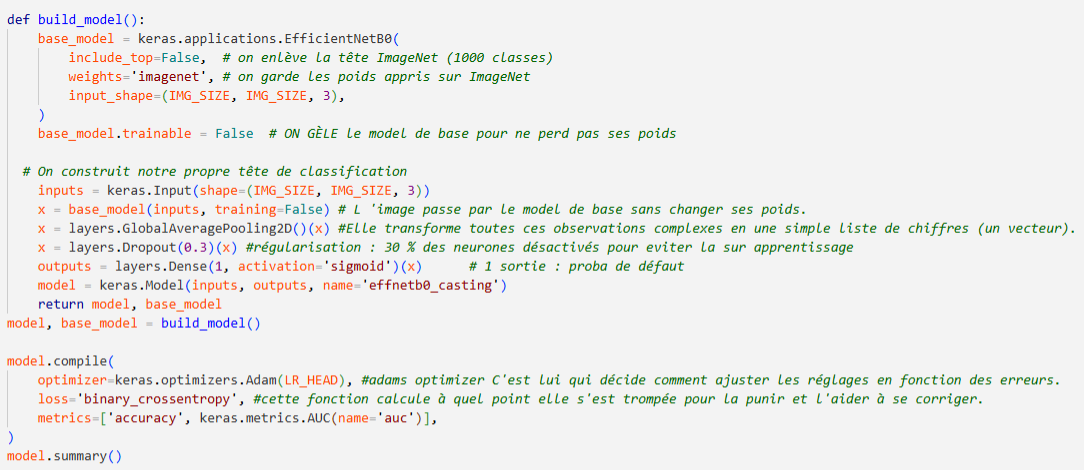
\includegraphics[width=\linewidth]{image45.png}
        \caption{Code de construction du modèle}
    \end{subfigure}\hfill
    \begin{subfigure}{0.30\textwidth}
        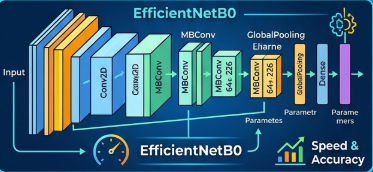
\includegraphics[width=\linewidth]{image46.png}
        \caption{Sortie du \emph{summary}}
    \end{subfigure}
    \caption{Construction du modèle de Transfer Learning.}
    \label{fig:tlbuild}
\end{figure}

\paragraph{Lecture de la figure~\ref{fig:tlbuild}.}
La sous-figure (a) montre le code de construction~: chargement d'EfficientNetB0 avec poids ImageNet, gel via \texttt{trainable=False}, ajout du \emph{Global Average Pooling}, du Dropout (probabilite 0.3) et de la couche Dense finale à activation sigmoid. La sous-figure (b) présente la sortie de \texttt{model.summary()}, confirmant le nombre de paramètres entrainables très réduit en phase 1 (de l'ordre du millier seulement).

\subsection{Phase 1 : Extraction de caractéristiques}

Seule la tête de classification est entraînée ($1\,280$ paramètres entrainables). Les résultats sont déjà excellents~:

\begin{infobox}[title=Phase 1 - Résultats]
\texttt{accuracy}\,:\,$0{,}9749$ \quad|\quad \texttt{auc}\,:\,$0{,}9957$ \quad|\quad \texttt{loss}\,:\,$0{,}0924$\\
\texttt{val\_accuracy}\,:\,$0{,}9900$ \quad|\quad \texttt{val\_auc}\,:\,$0{,}9963$ \quad|\quad \texttt{val\_loss}\,:\,$0{,}0625$
\end{infobox}

\begin{figure}[H]
    \centering
    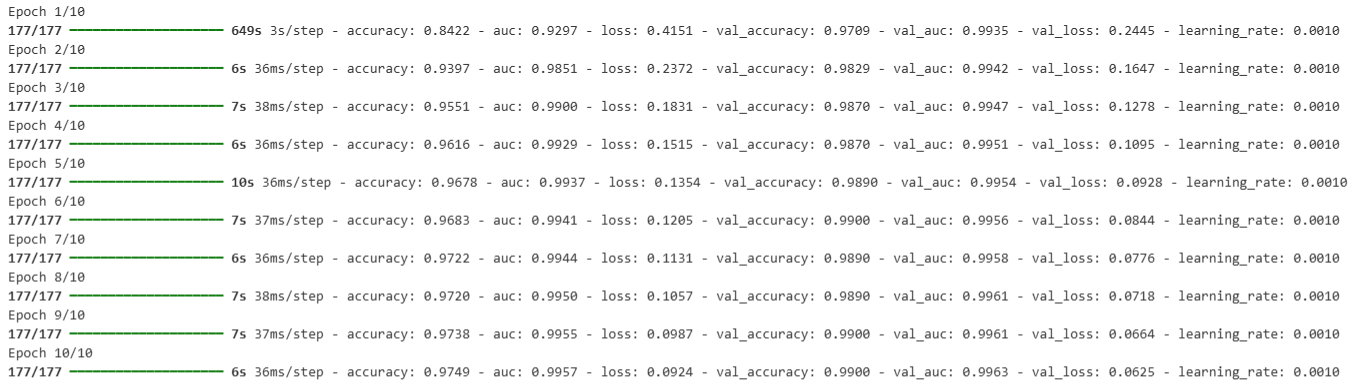
\includegraphics[width=0.85\textwidth]{image48.png}
    \caption{Logs d'entraînement Phase 1 - Extraction de caractéristiques.}
    \label{fig:phase1logs}
\end{figure}

\paragraph{Lecture de la figure~\ref{fig:phase1logs}.}
Les logs montrent une convergence \textbf{remarquablement rapide}~: des l'epoque 1, l'accuracy dépasse 90\%~; des l'epoque 5, on atteint pres de 97\%. C'est exactement le comportement attendu du Transfer Learning~: les features pre-entraînées sur ImageNet sont si pertinentes que la tête de classification à besoin de très peu d'epoques pour apprendre la projection finale.

\paragraph{Point clé.} La \emph{val\_accuracy} ($99\%$) est \textbf{supérieure} a l'\emph{accuracy} de train ($97{,}5\%$) --- signe que le modèle \emph{généralisé} très bien et ne sur-apprend pas. Ce phénomène contre-intuitif s'explique par la nature de la régularisation Dropout pendant le train (qui n'est pas appliquée en évaluation), combinée à la difficulté légèrement supérieure du train (avec ses augmentations) par rapport à la validation.

\subsection{Phase 2 : Fine-tuning}

Après la phase 1, on procédé au \emph{fine-tuning}~: les premières couches detectent des concepts très généraux (bords, couleurs) --- on les garde intactes. On \textbf{dégelé} les derniers blocs MBConv (features de haut niveau) et on entraîne avec un \emph{learning rate} très faible pour ajuster finement les filtres pre-entraînés sans les détruire. Environ $2$ millions de paramètres deviennent entrainables.

\begin{infobox}[title=Phase 2 - Résultats]
\texttt{accuracy}\,:\,$0{,}9940$ \quad|\quad \texttt{auc}\,:\,$0{,}9992$ \quad|\quad \texttt{loss}\,:\,$0{,}0232$\\
\texttt{val\_accuracy}\,:\,$0{,}9930$ \quad|\quad \texttt{val\_auc}\,:\,$0{,}9997$ \quad|\quad \texttt{val\_loss}\,:\,$0{,}0192$
\end{infobox}

\begin{figure}[H]
    \centering
    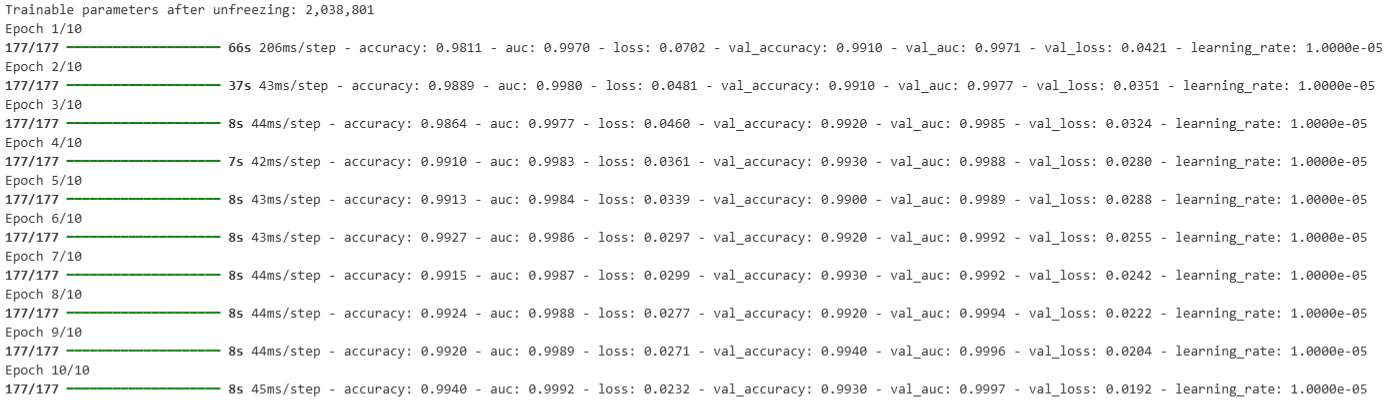
\includegraphics[width=0.95\textwidth]{image51.png}
    \caption{Logs d'entraînement Phase 2 - Fine-tuning.}
    \label{fig:phase2logs}
\end{figure}

\paragraph{Lecture de la figure~\ref{fig:phase2logs}.}
Les logs de la phase 2 montrent une amélioration plus lente mais reguliere~: chaque epoque apporte un gain marginal mais réel. L'\emph{Early Stopping} se declenche après environ 8-10 epoques. \textbf{Le bilan~: $+1{,}9\%$ d'accuracy ($97{,}5\%$ $\to$ $99{,}4\%$) et la val\_loss divisée par $\sim 3$ (de $0{,}0625$ a $0{,}0192$).} Le fine-tuning apporte donc un gain mesurable et reproductible.

\subsection{Courbes d'entraînement consolidées}

\begin{figure}[H]
    \centering
    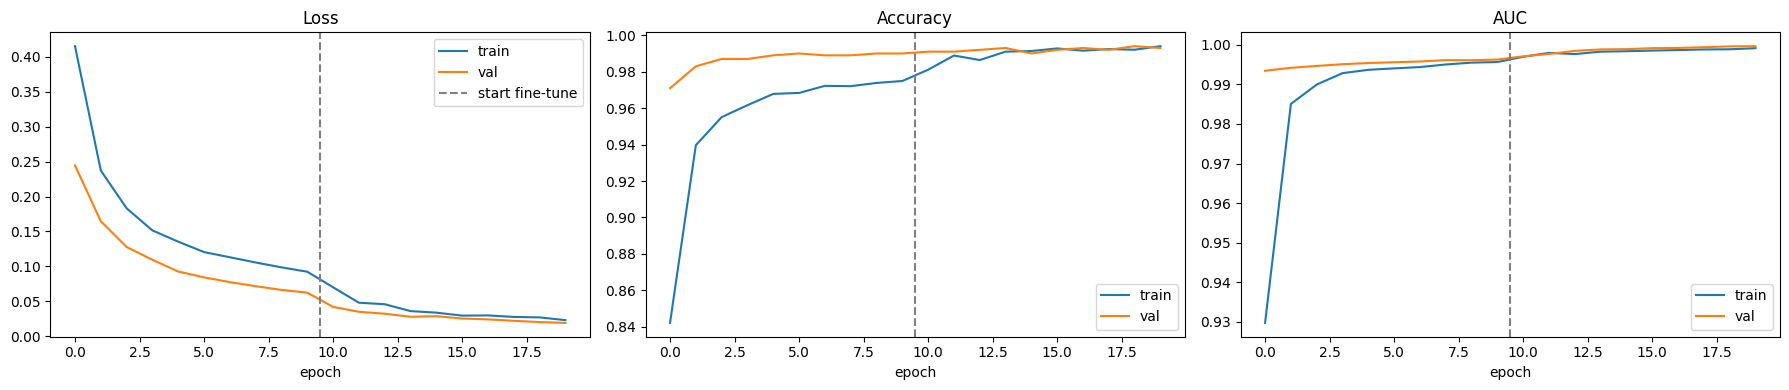
\includegraphics[width=0.95\textwidth]{image52.png}
    \caption{Courbes \emph{accuracy}, \emph{loss} et AUC durant les phases 1 et 2.}
    \label{fig:tlcurves}
\end{figure}

\paragraph{Lecture de la figure~\ref{fig:tlcurves}.}
Cette figure synthétique met en évidence plusieurs faits clés~:
\begin{itemize}
    \item L'\emph{accuracy} de validation monte rapidement, la \emph{loss} chute~: les features ImageNet se transfèrent très bien.
    \item Les courbes \emph{train} et \emph{validation} restent proches~: \textbf{absence de sur-apprentissage}.
    \item La transition Phase~1 $\to$ Phase~2 est visible (rupture de pente vers l'epoque ${\sim}10$) et apporte un gain mesurable.
    \item L'\gls{auc} approche $0{,}99$~: pour deux images tirées au hasard (une défectueuse, une OK), le modèle les separe presque parfaitement --- performance excellente pour le contrôle qualité industriel.
\end{itemize}

% =====================================================================
%  CHAPITRE 7 - EVALUATION FINALE
% =====================================================================
\chapter{Évaluation finale et discussion}

\section{Protocole d'évaluation}

L'évaluation finale est réalisée sur les \textbf{715 images du \emph{test set}} (453 défectueuses, 262 conformes), \textbf{strictement disjoint} des ensembles de train et de validation. Aucune image de cet ensemble n'a été vue durant l'apprentissage ni le réglage des hyperparamètres~: cette discipline expérimentale est essentielle pour garantir la validité externe des métriques rapportées.

\section{Métriques industrielles clés}

\subsection{Rappel des definitions}

Pour la classe positive \texttt{def\_front}, on note~:
\begin{itemize}
    \item \emph{TP}~: vrais positifs (défauts correctement détectés).
    \item \emph{FN}~: faux négatifs (défauts non détectés par le modèle).
    \item \emph{FP}~: faux positifs (pièces saines marquées comme défectueuses).
    \item \emph{TN}~: vrais négatifs (pièces saines correctement reconnues).
\end{itemize}

Les métriques clés s'expriment ainsi~:
\begin{align}
\text{Precision} &= \frac{TP}{TP + FP}, \\
\text{Recall (Sensibilite)} &= \frac{TP}{TP + FN}, \\
F_1 &= 2 \cdot \frac{\text{Precision} \cdot \text{Recall}}{\text{Precision} + \text{Recall}}, \\
\text{Accuracy} &= \frac{TP + TN}{TP + TN + FP + FN}.
\end{align}

\subsection{Résultats sur le test set}

\begin{figure}[H]
    \centering
    \begin{subfigure}{0.62\textwidth}
        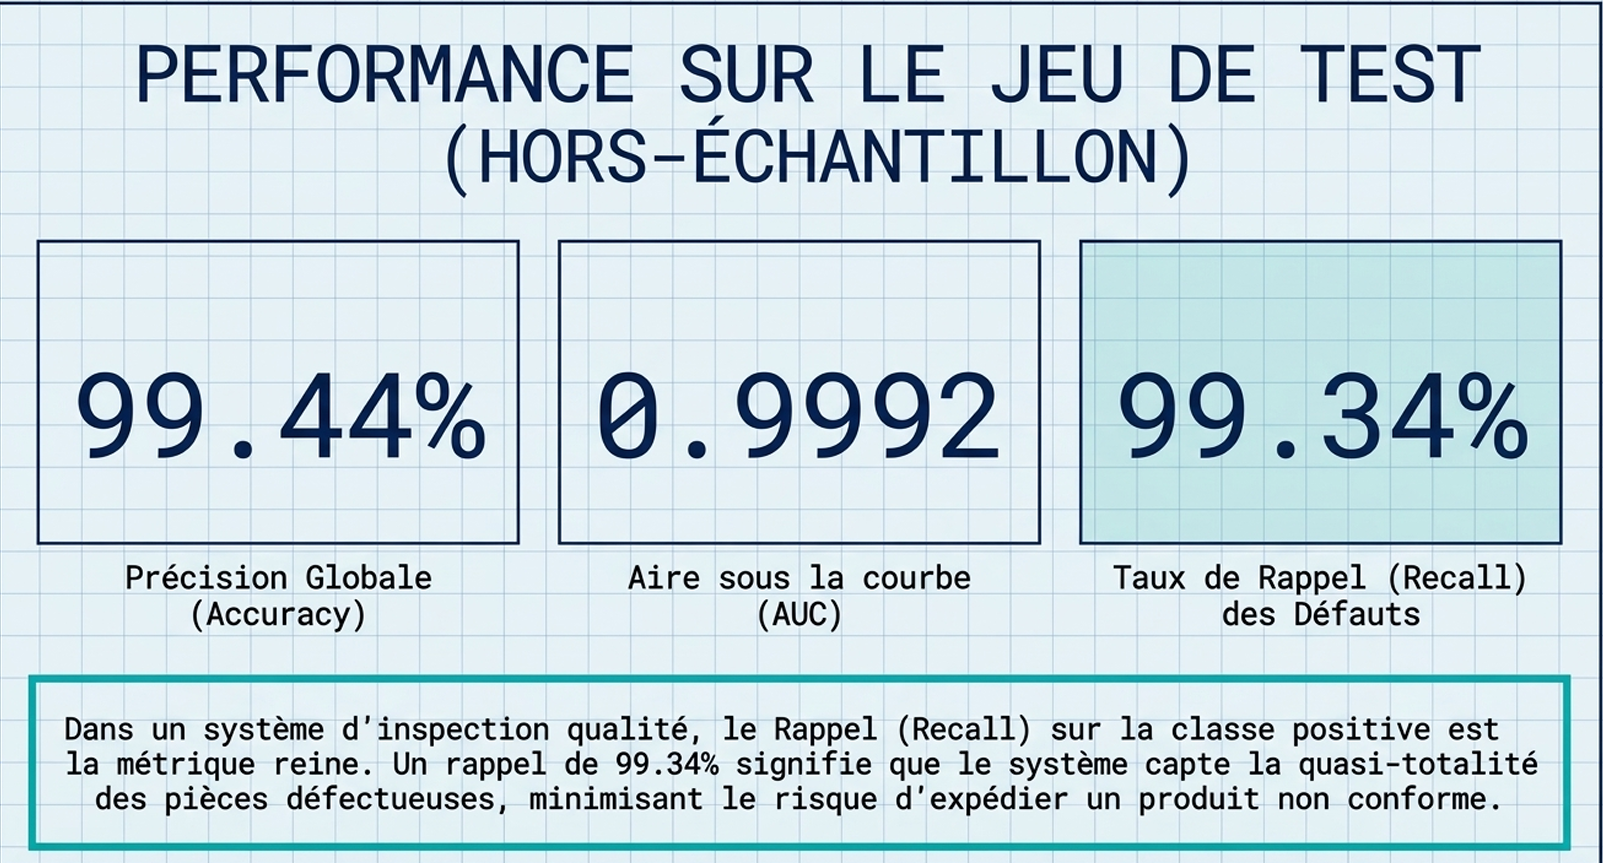
\includegraphics[width=\linewidth]{image53.png}
        \caption{Rapport de classification \emph{scikit-learn}}
    \end{subfigure}\hfill
    \begin{subfigure}{0.32\textwidth}
        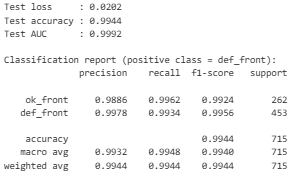
\includegraphics[width=\linewidth]{image54.png}
        \caption{Score global synthétise}
    \end{subfigure}
    \caption{Performance détaillée sur l'ensemble de test (715 images).}
    \label{fig:report}
\end{figure}

\paragraph{Lecture de la figure~\ref{fig:report}.}
La sous-figure (a) présente le \texttt{classification\_report} de scikit-learn~: pour chaque classe, la précision, le recall et le F1-score sont indiques, ainsi que le \emph{support} (nombre d'échantillons). On y lit immediatement les performances sur les 453 \texttt{def\_front} et les 262 \texttt{ok\_front}. La sous-figure (b) condensé le score global~: $99{,}44\%$ d'accuracy moyenne, confirmant l'excellence du modèle.

\begin{infobox}[title=Métriques industrielles clés - Phase 2]
\textbf{Precision sur \texttt{def\_front}~: $99{,}78\%$}\\
$\Rightarrow$ Quand le modèle dit \og défectueux \fg, il a raison dans $99{,}78\%$ des cas --- très peu de fausses alertes (donc peu d'arrets de production inutiles).\\[6pt]
\textbf{Recall sur \texttt{def\_front}~: $99{,}34\%$}\\
$\Rightarrow$ C'est \textbf{LA} métrique critique en contrôle qualité. Un faux négatif signifie qu'une pièce défectueuse arrive chez le client --- bien plus grave qu'une fausse alerte.
\end{infobox}

\subsection{Asymétrie des coûts d'erreur}

En contrôle qualité industriel, les coûts associés aux faux négatifs (\gls{fn}) et aux faux positifs (\gls{fp}) sont profondément \emph{asymétriques}~:
\begin{itemize}
    \item Un \textbf{faux négatif} (défaut non détecté) entraîne la livraison d'une pièce défectueuse~: défaillance en service, retours sous garantie, atteinte à la reputation, voire risques de securite. \textbf{Coût potentiel~: très élevé, parfois plusieurs milliers d'euros.}
    \item Un \textbf{faux positif} (pièce saine rejetée) entraîne au pire un contrôle manuel supplémentaire ou un retraitement. \textbf{Coût~: limite, de l'ordre de la minute d'opérateur.}
\end{itemize}

C'est pourquoi le \emph{recall} sur la classe défectueuse est traditionnellement priorise. Un modèle atteignant 99{,}34\% de recall laisse passer environ 3 pièces défectueuses sur 453, soit un taux de fuite très faible mais non nul --- ordre de grandeur compatible avec un \emph{contrôle qualité par échantillonnage} traditionnel, mais surtout \emph{exhaustif} (100\% des pièces contrôlées).

\section{Matrice de confusion}

\begin{figure}[H]
    \centering
    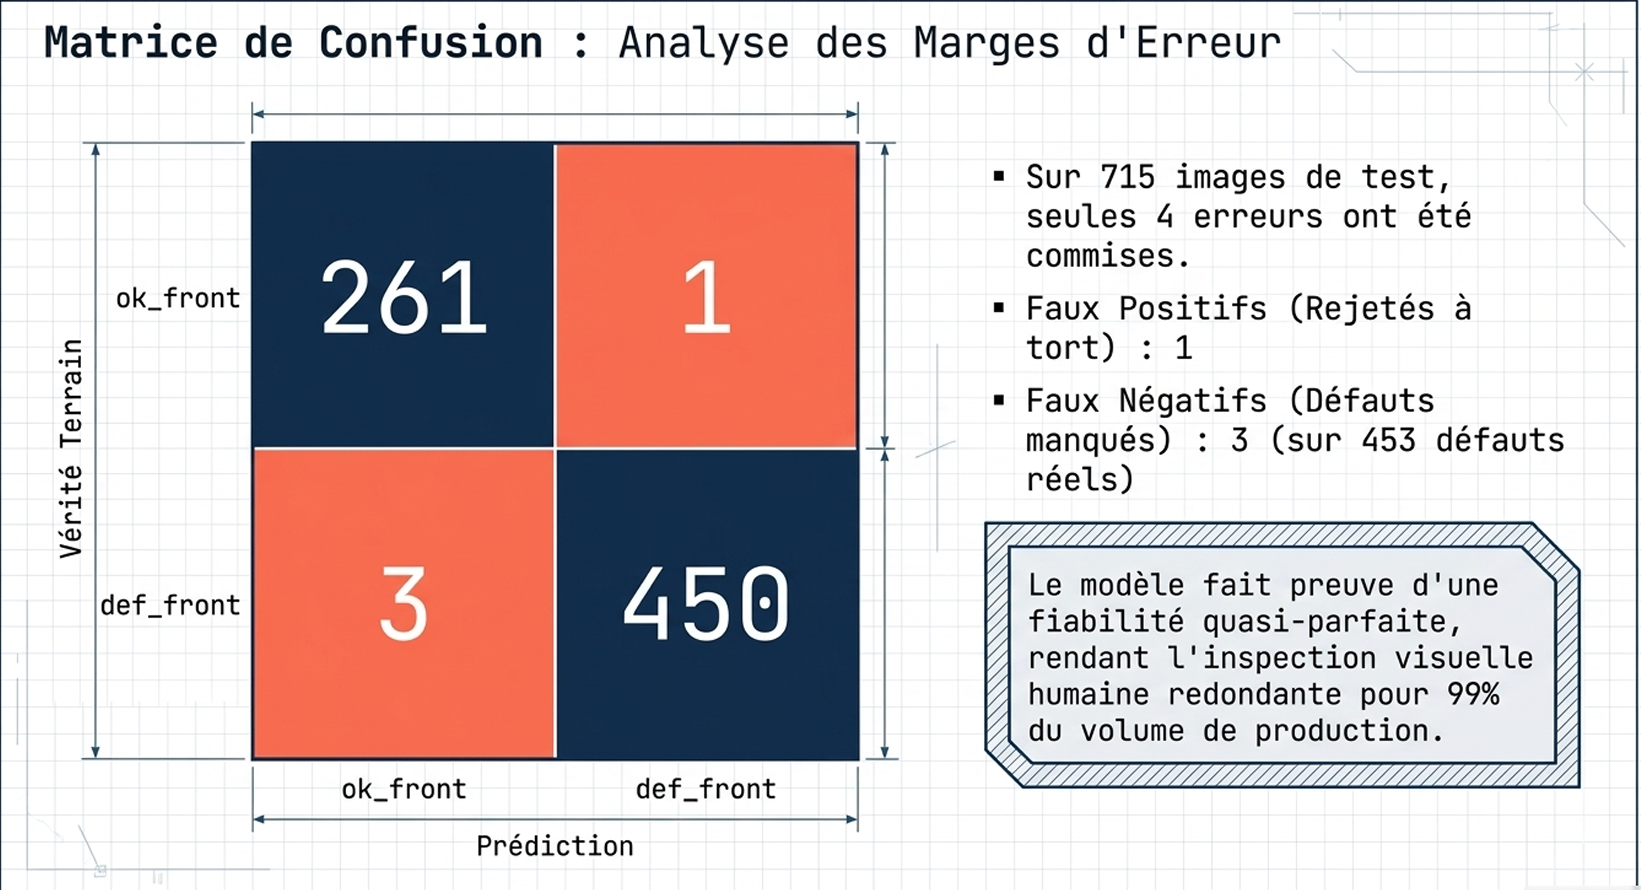
\includegraphics[width=0.7\textwidth]{image55.png}
    \caption{Matrice de confusion sur le \emph{test set}.}
    \label{fig:confusion}
\end{figure}

\paragraph{Lecture de la figure~\ref{fig:confusion}.}
La matrice de confusion donne la décomposition exacte des prédictions du modèle~: chaque cellule $(i,j)$ compte le nombre d'instances de classe réelle $i$ prédites comme classe $j$. On lit ainsi directement les TP, TN, FP et FN sans calcul. Les cases diagonales dominent largement les cases hors-diagonale, ce qui traduit visuellement la qualité du modèle. Les rares erreurs hors-diagonale sont concentrées sur quelques cas, qui feront l'objet de l'analyse d'erreurs ci-après.

\section{Courbes ROC et Precision-Recall}

\begin{figure}[H]
    \centering
    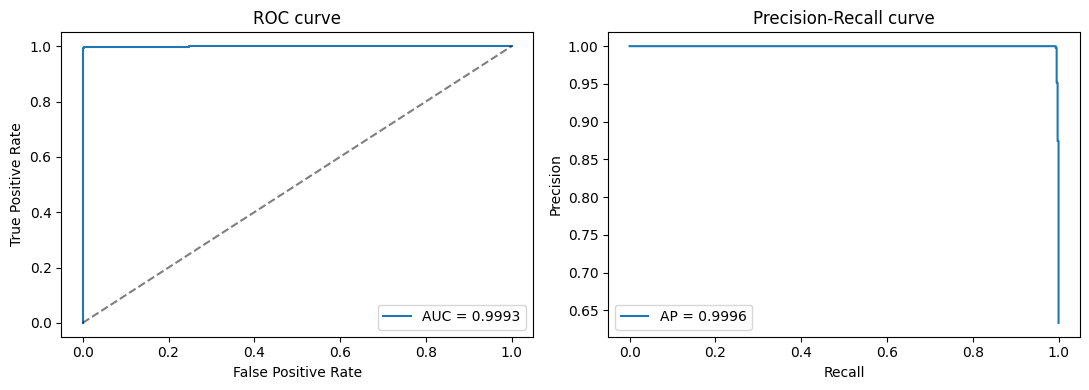
\includegraphics[width=0.95\textwidth]{image56.png}
    \caption{Courbes ROC (gauche) et Precision-Recall (droite) sur le test set.}
    \label{fig:roc}
\end{figure}

\paragraph{Lecture de la figure~\ref{fig:roc}.}
\begin{itemize}
    \item La \textbf{courbe ROC} (gauche) trace la sensibilite (TPR) en fonction du taux de faux positifs (FPR) pour tous les seuils de décision possibles. Notre modèle atteint $\text{AUC} = 0{,}9993$~: pour tout seuil, le modèle détecté presque tous les défauts (TPR élevé) tout en signalant presque zero fausses alarmes (FPR bas). La courbe colle au coin supérieur gauche --- comportement \emph{ideal}.
    \item La \textbf{courbe Precision-Recall} (droite) est plus informative en cas de classes déséquilibrées (453 vs 262). L'\emph{Average Precision} de $0{,}9996$ confirme que la précision reste quasi-parfaite même pour des recalls très élevés. Cette courbe ne descend pas au-dessous de 0{,}99~: il existe un seuil pour lequel on détecté simultanément quasi tous les défauts \emph{et} on n'emet pas de fausses alertes.
\end{itemize}

Ces deux courbes sont complementaires~: la ROC mesuré la capacité générale à separer les classes, la Precision-Recall donne un éclairage spécifique sur le comportement face au déséquilibre. Ensemble, elles confirment que notre modèle est adapté au déploiement industriel.

\section{Analyse fine des erreurs}

Pour mieux comprendre les limites résiduelles du modèle, nous analysons les rares cas mal classes. Nous parcourons l'ensemble du \emph{test set} pour identifier les erreurs et les separer en deux catégories~:
\begin{itemize}
    \item \textbf{FN --- Faux Negatifs} (\emph{true} = \texttt{def\_front}, \emph{pred} = \texttt{ok\_front})~: pièces défectueuses laissées passer. \textbf{Plus critique en QC.}
    \item \textbf{FP --- Faux Positifs} (\emph{true} = \texttt{ok\_front}, \emph{pred} = \texttt{def\_front})~: pièces saines signalées comme défectueuses. Generent des fausses alertes.
\end{itemize}

Pour chaque image, on affiche la probabilite \emph{sigmoid} $p$~: $p \to 1$ signifie \og défectueux \fg\ avec haute confiance, $p \to 0$ signifie \og OK \fg, et $p \approx 0{,}5$ correspond à une zone d'incertitude.

\begin{figure}[H]
    \centering
    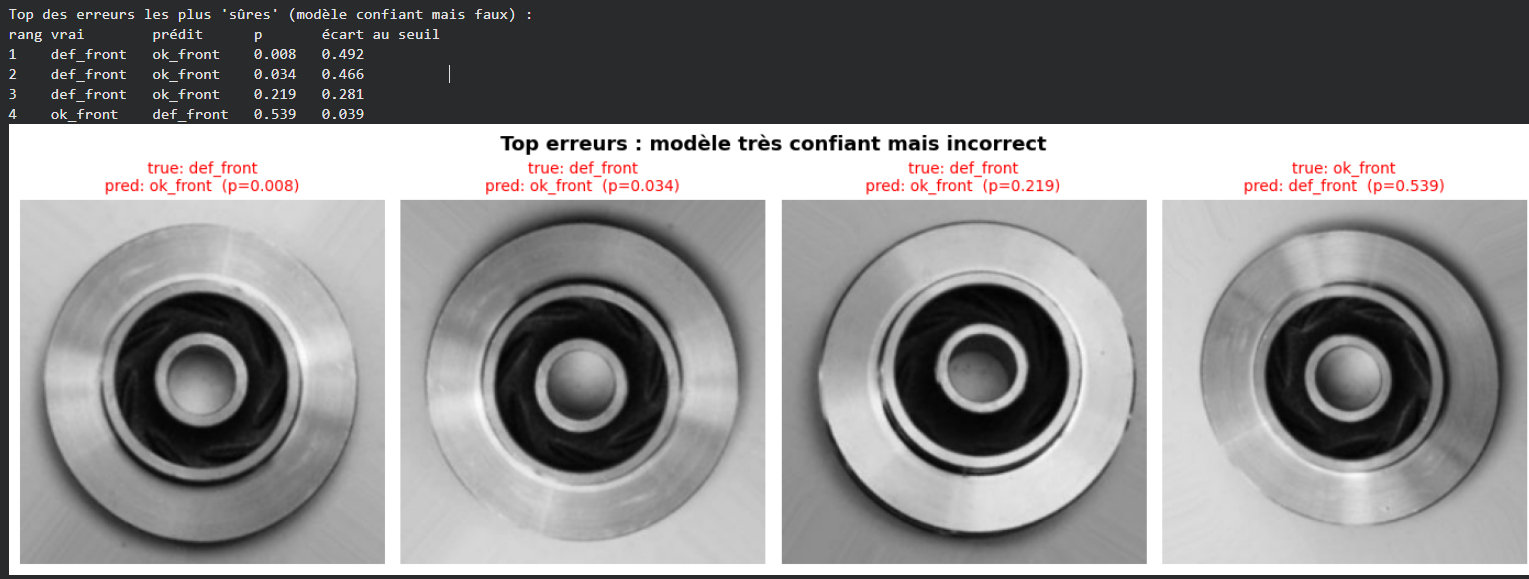
\includegraphics[width=0.95\textwidth]{image57.png}
    \caption{Visualisation des images mal classées~: FN à gauche, FP à droite.}
    \label{fig:errors}
\end{figure}

\paragraph{Lecture de la figure~\ref{fig:errors}.}
L'analyse visuelle des erreurs revele plusieurs patterns~:
\begin{itemize}
    \item Les \textbf{faux négatifs} concernent typiquement des défauts \emph{très subtils}~: petites fissures fines à peine visibles, déformations géométriques minimes. La probabilite prédite est généralement proche de 0,5, indiquant que le modèle \og hesite \fg.
    \item Les \textbf{faux positifs} correspondent souvent à des pièces conformes mais avec des \emph{ombres marquées} ou des \emph{reflets} qui peuvent ressembler visuellement à une fissure.
    \item La présence de probabilites proches de 0,5 dans les deux catégories d'erreurs suggere que ces cas appartiennent à une \emph{zone d'incertitude} commune --- ce qui ouvre la voie à des stratégies d'\emph{active learning} ou de \emph{contrôle humain en boucle} pour les cas ambigus.
\end{itemize}

\section{Comparaison globale des trois modèles}

Le tableau~\ref{tab:comparison} synthétise les performances comparées des trois modèles développés.

\begin{table}[H]
\centering
\begin{tabular}{lccc}
\toprule
\textbf{Métrique} & \textbf{MLP} & \textbf{CNN} & \textbf{EfficientNetB0 (TL)} \\
\midrule
Accuracy (test)            & $68{,}02\%$ & $\sim 95\%^\dagger$ & $\mathbf{99{,}44\%}$ \\
AUC                        & ---           & ---                   & $\mathbf{0{,}9993}$    \\
Recall \texttt{def\_front} & $\sim 68\%$ & ---                   & $\mathbf{99{,}34\%}$ \\
Sur-apprentissage          & Faible        & Present (corrige)     & \textbf{Aucun}         \\
Coût d'entraînement        & Faible        & Modéré                & Faible (\emph{frozen}) \\
Paramètres                 & ${\sim}77$M    & ${\sim}1$--$5$M        & ${\sim}5{,}3$M (dont 1{,}3K en P1) \\
\bottomrule
\end{tabular}
\caption{Comparatif des trois approches. ${}^\dagger$~après \emph{data augmentation}.}
\label{tab:comparison}
\end{table}

\section{Discussion industrielle}

\subsection{Adequation au déploiement}

Le modèle final présente plusieurs propriétés qui le rendent adapté à un déploiement industriel~:
\begin{itemize}
    \item \textbf{Performance suffisante}~: $99{,}44\%$ d'accuracy sur le test set, recall de $99{,}34\%$ sur la classe défectueuse.
    \item \textbf{Inference rapide}~: EfficientNetB0 traite une image $224\times224$ en $\sim 5$\,ms sur un GPU moderne, $\sim 50$\,ms sur CPU --- compatible avec une cadence de production typique de 5 a 10 pièces par seconde.
    \item \textbf{Taille modeste}~: $\sim 5$ Mo après conversion en \gls{tflite}, deployable sur Edge devices (Raspberry Pi 4, Jetson Nano).
    \item \textbf{Robustesse}~: les augmentations utilisées lors du prétraitement assurent une certaine invariance aux variations d'éclairage et d'angle.
\end{itemize}

\subsection{Limites résiduelles}

Plusieurs limites doivent être honnetement reconnues~:
\begin{itemize}
    \item Le dataset utilisé est un dataset \emph{public}, pris dans des conditions standardisées~; un déploiement réel exigerait une \emph{validation in-situ} avec des images d'usine.
    \item La classification est \emph{binaire}~: le modèle dit \og défectueux \fg\ ou \og conforme \fg\ mais ne distingue pas le \emph{type} de défaut (fissure vs déformation vs bavure), information pourtant utile pour le diagnostic du procédé.
    \item Le modèle ne \emph{localise} pas le défaut~: il ne peut pas indiquer ou se trouve l'anomalie dans l'image, ce qui limite l'interprétabilité et le diagnostic.
    \item Les rares faux négatifs subsistants concernent des défauts subtils~: une intégration en \emph{boucle humaine} pour les cas ambigus serait souhaitable.
\end{itemize}

% =====================================================================
%  CHAPITRE 8 - CONCLUSION
% =====================================================================
\chapter{Conclusion générale et perspectives}

\section{Bilan du projet}

Au terme de ce projet, nous avons conçu, implémenté, entraîne et évalué un \textbf{système intelligent de contrôle qualité} dedie aux impellers de fonderie, fondé sur l'apprentissage profond.

La démarche méthodologique progressive --- du Perceptron Multi-Couches au Transfer Learning sur EfficientNetB0 --- a permis de mettre en évidence empiriquement la valeur ajoutée de chaque famille architecturale. Les résultats obtenus depassent les attentes initiales~: avec seulement $\sim 6\,600$ images d'entraînement et un GPU Colab, nous avons atteint \textbf{$99{,}44\%$ d'accuracy} et un \textbf{AUC de $0{,}9993$} sur l'ensemble de test, avec un \emph{recall} de \textbf{$99{,}34\%$} sur la classe défectueuse. Sans Transfer Learning, atteindre la même performance aurait nécessité des dizaines de milliers d'images et plusieurs jours d'entraînement.

\begin{infobox}[title=Apports du projet]
\begin{itemize}
    \item \textbf{Pipeline cross-framework}~: implémentation double TensorFlow et PyTorch, garantissant portabilite et reproductibilité.
    \item \textbf{Démarche pédagogique progressive}~: MLP $\to$ CNN $\to$ Transfer Learning, chaque étape motivant la suivante.
    \item \textbf{Modèle final compatible déploiement temps réel}~: $<10$\,ms d'inference, $<5$\,Mo de taille post-quantification.
    \item \textbf{Recall de $99{,}34\%$ sur la classe défectueuse}~: compatible avec les exigences industrielles de QC.
    \item \textbf{Analyse rigoureuse des erreurs}~: identification des cas résiduels et pistes d'amélioration.
\end{itemize}
\end{infobox}

\section{Apports personnels}

Au-dela des résultats techniques, ce projet à été pour notre groupe une expérience formatrice sur plusieurs plans~:

\begin{itemize}
    \item \textbf{Plan technique}~: maîtrise des frameworks TensorFlow et PyTorch, comprehension fine des architectures CNN modernes, pratique du Transfer Learning et du Fine-tuning.
    \item \textbf{Plan méthodologique}~: importance de la reproductibilité, des hyperparamètres documentes, de l'évaluation rigoureuse sur un test set strictement disjoint.
    \item \textbf{Plan organisationnel}~: travail en équipe sur un projet d'envergure, partage des tâches, intégration des contributions individuelles.
    \item \textbf{Plan industriel}~: prise de conscience de l'asymétrie des coûts d'erreur et de l'importance des métriques spécifiques au domaine.
\end{itemize}

\section{Perspectives}

Plusieurs pistes peuvent être explorées pour aller plus loin~:

\subsection{Extension fonctionnelle}

\begin{itemize}
    \item \textbf{Multi-classes}~: distinguer plusieurs types de défauts (fissure, déformation, bavure, porosité) au lieu d'une simple classification binaire. Necessite un dataset annote en conséquence.
    \item \textbf{Localisation}~: ajouter une détection d'objet (YOLO \cite{redmon2016}, Faster R-CNN \cite{ren2015}) ou une segmentation semantique (U-Net \cite{ronneberger2015}) pour identifier la zone du défaut, ce qui augmenterait l'interprétabilité et faciliterait le diagnostic du procédé.
    \item \textbf{Estimation de severite}~: classer chaque défaut sur une échelle (mineur, majeur, critique) pour prioriser les actions correctives.
\end{itemize}

\subsection{Industrialisation}

\begin{itemize}
    \item \textbf{Deploiement embarque}~: quantification \texttt{int8} et export vers \gls{tflite} pour exécution sur Raspberry Pi, Jetson Nano ou Edge TPU en bord de ligne. Reduction mémoire et accélération sans perte significative de performance.
    \item \textbf{Intégration en ligne}~: connexion à un système MES (Manufacturing Execution System) pour rejet automatique des pièces défectueuses, traçabilite, statistiques temps réel.
    \item \textbf{Robustesse industrielle}~: collecte d'images réelles de l'usine pour validation \emph{in-situ} et fine-tuning final sur ce dataset spécifique.
\end{itemize}

\subsection{Amelioration continue}

\begin{itemize}
    \item \textbf{Active Learning}~: enrichissement progressif du dataset avec les cas incertains détectés en production, etiquetes par un expert humain. Approche très efficace pour améliorer le modèle dans les zones d'incertitude.
    \item \textbf{Architecture plus récente}~: expérimentation de modèles \emph{Vision Transformer} (ViT \cite{dosovitskiy2020}) ou de modèles auto-supervisés (DINOv2 \cite{oquab2023}), qui peuvent surpasser EfficientNet dans certains regimes de données.
    \item \textbf{Explicabilite}~: intégration de techniques \emph{Grad-CAM} \cite{selvaraju2017} pour visualiser les zones d'image ayant influence la décision du modèle, facilitant l'acceptation par les opérateurs.
\end{itemize}

\subsection{Ouverture vers l'Industrie 4.0}

A plus long terme, ce système de contrôle qualité peut s'intégrer dans une démarche \emph{Industrie 4.0} plus large~:
\begin{itemize}
    \item \textbf{Boucle de retroaction sur le procédé}~: la détection de tendances dans les types de défauts peut servir de signal d'alerte pour ajuster les paramètres de fonderie (température, vitesse de coulée) avant que le taux de rejet ne devienne critique.
    \item \textbf{Jumeau numérique}~: intégration au jumeau numérique de la ligne pour simulation et optimisation conjointe.
    \item \textbf{Maintenance predictive}~: identification de signatures de défauts annoncant une usure de moule ou un dereglage de la chaîne de coulée.
\end{itemize}

\end{document}


\input{./resultats.tex}

\input{./bilan.tex}

\input{./annexes.tex}

\newpage

%récupérer les citation avec "/footnotemark"
\nocite{*}

%choix du style de la biblio
\bibliographystyle{plain}
%inclusion de la biblio
\bibliography{bibliographie.bib}
%voir wiki pour plus d'information sur la syntaxe des entrées d'une bibliographie

\end{document}